% Options for packages loaded elsewhere
% Options for packages loaded elsewhere
\PassOptionsToPackage{unicode}{hyperref}
\PassOptionsToPackage{hyphens}{url}
\PassOptionsToPackage{dvipsnames,svgnames,x11names}{xcolor}
%
\documentclass[
  letterpaper,
  DIV=11,
  numbers=noendperiod]{scrartcl}
\usepackage{xcolor}
\usepackage{amsmath,amssymb}
\setcounter{secnumdepth}{5}
\usepackage{iftex}
\ifPDFTeX
  \usepackage[T1]{fontenc}
  \usepackage[utf8]{inputenc}
  \usepackage{textcomp} % provide euro and other symbols
\else % if luatex or xetex
  \usepackage{unicode-math} % this also loads fontspec
  \defaultfontfeatures{Scale=MatchLowercase}
  \defaultfontfeatures[\rmfamily]{Ligatures=TeX,Scale=1}
\fi
\usepackage{lmodern}
\ifPDFTeX\else
  % xetex/luatex font selection
\fi
% Use upquote if available, for straight quotes in verbatim environments
\IfFileExists{upquote.sty}{\usepackage{upquote}}{}
\IfFileExists{microtype.sty}{% use microtype if available
  \usepackage[]{microtype}
  \UseMicrotypeSet[protrusion]{basicmath} % disable protrusion for tt fonts
}{}
\makeatletter
\@ifundefined{KOMAClassName}{% if non-KOMA class
  \IfFileExists{parskip.sty}{%
    \usepackage{parskip}
  }{% else
    \setlength{\parindent}{0pt}
    \setlength{\parskip}{6pt plus 2pt minus 1pt}}
}{% if KOMA class
  \KOMAoptions{parskip=half}}
\makeatother
% Make \paragraph and \subparagraph free-standing
\makeatletter
\ifx\paragraph\undefined\else
  \let\oldparagraph\paragraph
  \renewcommand{\paragraph}{
    \@ifstar
      \xxxParagraphStar
      \xxxParagraphNoStar
  }
  \newcommand{\xxxParagraphStar}[1]{\oldparagraph*{#1}\mbox{}}
  \newcommand{\xxxParagraphNoStar}[1]{\oldparagraph{#1}\mbox{}}
\fi
\ifx\subparagraph\undefined\else
  \let\oldsubparagraph\subparagraph
  \renewcommand{\subparagraph}{
    \@ifstar
      \xxxSubParagraphStar
      \xxxSubParagraphNoStar
  }
  \newcommand{\xxxSubParagraphStar}[1]{\oldsubparagraph*{#1}\mbox{}}
  \newcommand{\xxxSubParagraphNoStar}[1]{\oldsubparagraph{#1}\mbox{}}
\fi
\makeatother

\usepackage{color}
\usepackage{fancyvrb}
\newcommand{\VerbBar}{|}
\newcommand{\VERB}{\Verb[commandchars=\\\{\}]}
\DefineVerbatimEnvironment{Highlighting}{Verbatim}{commandchars=\\\{\}}
% Add ',fontsize=\small' for more characters per line
\usepackage{framed}
\definecolor{shadecolor}{RGB}{241,243,245}
\newenvironment{Shaded}{\begin{snugshade}}{\end{snugshade}}
\newcommand{\AlertTok}[1]{\textcolor[rgb]{0.68,0.00,0.00}{#1}}
\newcommand{\AnnotationTok}[1]{\textcolor[rgb]{0.37,0.37,0.37}{#1}}
\newcommand{\AttributeTok}[1]{\textcolor[rgb]{0.40,0.45,0.13}{#1}}
\newcommand{\BaseNTok}[1]{\textcolor[rgb]{0.68,0.00,0.00}{#1}}
\newcommand{\BuiltInTok}[1]{\textcolor[rgb]{0.00,0.23,0.31}{#1}}
\newcommand{\CharTok}[1]{\textcolor[rgb]{0.13,0.47,0.30}{#1}}
\newcommand{\CommentTok}[1]{\textcolor[rgb]{0.37,0.37,0.37}{#1}}
\newcommand{\CommentVarTok}[1]{\textcolor[rgb]{0.37,0.37,0.37}{\textit{#1}}}
\newcommand{\ConstantTok}[1]{\textcolor[rgb]{0.56,0.35,0.01}{#1}}
\newcommand{\ControlFlowTok}[1]{\textcolor[rgb]{0.00,0.23,0.31}{\textbf{#1}}}
\newcommand{\DataTypeTok}[1]{\textcolor[rgb]{0.68,0.00,0.00}{#1}}
\newcommand{\DecValTok}[1]{\textcolor[rgb]{0.68,0.00,0.00}{#1}}
\newcommand{\DocumentationTok}[1]{\textcolor[rgb]{0.37,0.37,0.37}{\textit{#1}}}
\newcommand{\ErrorTok}[1]{\textcolor[rgb]{0.68,0.00,0.00}{#1}}
\newcommand{\ExtensionTok}[1]{\textcolor[rgb]{0.00,0.23,0.31}{#1}}
\newcommand{\FloatTok}[1]{\textcolor[rgb]{0.68,0.00,0.00}{#1}}
\newcommand{\FunctionTok}[1]{\textcolor[rgb]{0.28,0.35,0.67}{#1}}
\newcommand{\ImportTok}[1]{\textcolor[rgb]{0.00,0.46,0.62}{#1}}
\newcommand{\InformationTok}[1]{\textcolor[rgb]{0.37,0.37,0.37}{#1}}
\newcommand{\KeywordTok}[1]{\textcolor[rgb]{0.00,0.23,0.31}{\textbf{#1}}}
\newcommand{\NormalTok}[1]{\textcolor[rgb]{0.00,0.23,0.31}{#1}}
\newcommand{\OperatorTok}[1]{\textcolor[rgb]{0.37,0.37,0.37}{#1}}
\newcommand{\OtherTok}[1]{\textcolor[rgb]{0.00,0.23,0.31}{#1}}
\newcommand{\PreprocessorTok}[1]{\textcolor[rgb]{0.68,0.00,0.00}{#1}}
\newcommand{\RegionMarkerTok}[1]{\textcolor[rgb]{0.00,0.23,0.31}{#1}}
\newcommand{\SpecialCharTok}[1]{\textcolor[rgb]{0.37,0.37,0.37}{#1}}
\newcommand{\SpecialStringTok}[1]{\textcolor[rgb]{0.13,0.47,0.30}{#1}}
\newcommand{\StringTok}[1]{\textcolor[rgb]{0.13,0.47,0.30}{#1}}
\newcommand{\VariableTok}[1]{\textcolor[rgb]{0.07,0.07,0.07}{#1}}
\newcommand{\VerbatimStringTok}[1]{\textcolor[rgb]{0.13,0.47,0.30}{#1}}
\newcommand{\WarningTok}[1]{\textcolor[rgb]{0.37,0.37,0.37}{\textit{#1}}}

\usepackage{longtable,booktabs,array}
\usepackage{calc} % for calculating minipage widths
% Correct order of tables after \paragraph or \subparagraph
\usepackage{etoolbox}
\makeatletter
\patchcmd\longtable{\par}{\if@noskipsec\mbox{}\fi\par}{}{}
\makeatother
% Allow footnotes in longtable head/foot
\IfFileExists{footnotehyper.sty}{\usepackage{footnotehyper}}{\usepackage{footnote}}
\makesavenoteenv{longtable}
\usepackage{graphicx}
\makeatletter
\newsavebox\pandoc@box
\newcommand*\pandocbounded[1]{% scales image to fit in text height/width
  \sbox\pandoc@box{#1}%
  \Gscale@div\@tempa{\textheight}{\dimexpr\ht\pandoc@box+\dp\pandoc@box\relax}%
  \Gscale@div\@tempb{\linewidth}{\wd\pandoc@box}%
  \ifdim\@tempb\p@<\@tempa\p@\let\@tempa\@tempb\fi% select the smaller of both
  \ifdim\@tempa\p@<\p@\scalebox{\@tempa}{\usebox\pandoc@box}%
  \else\usebox{\pandoc@box}%
  \fi%
}
% Set default figure placement to htbp
\def\fps@figure{htbp}
\makeatother





\setlength{\emergencystretch}{3em} % prevent overfull lines

\providecommand{\tightlist}{%
  \setlength{\itemsep}{0pt}\setlength{\parskip}{0pt}}



 


\usepackage{booktabs}
\usepackage{longtable}
\usepackage{array}
\usepackage{multirow}
\usepackage{wrapfig}
\usepackage{float}
\usepackage{colortbl}
\usepackage{pdflscape}
\usepackage{tabu}
\usepackage{threeparttable}
\usepackage{threeparttablex}
\usepackage[normalem]{ulem}
\usepackage{makecell}
\usepackage{xcolor}
\KOMAoption{captions}{tableheading,figureheading}
\makeatletter
\@ifpackageloaded{caption}{}{\usepackage{caption}}
\AtBeginDocument{%
\ifdefined\contentsname
  \renewcommand*\contentsname{Table of contents}
\else
  \newcommand\contentsname{Table of contents}
\fi
\ifdefined\listfigurename
  \renewcommand*\listfigurename{List of Figures}
\else
  \newcommand\listfigurename{List of Figures}
\fi
\ifdefined\listtablename
  \renewcommand*\listtablename{List of Tables}
\else
  \newcommand\listtablename{List of Tables}
\fi
\ifdefined\figurename
  \renewcommand*\figurename{Figure}
\else
  \newcommand\figurename{Figure}
\fi
\ifdefined\tablename
  \renewcommand*\tablename{Table}
\else
  \newcommand\tablename{Table}
\fi
}
\@ifpackageloaded{float}{}{\usepackage{float}}
\floatstyle{ruled}
\@ifundefined{c@chapter}{\newfloat{codelisting}{h}{lop}}{\newfloat{codelisting}{h}{lop}[chapter]}
\floatname{codelisting}{Listing}
\newcommand*\listoflistings{\listof{codelisting}{List of Listings}}
\makeatother
\makeatletter
\makeatother
\makeatletter
\@ifpackageloaded{caption}{}{\usepackage{caption}}
\@ifpackageloaded{subcaption}{}{\usepackage{subcaption}}
\makeatother
\usepackage{bookmark}
\IfFileExists{xurl.sty}{\usepackage{xurl}}{} % add URL line breaks if available
\urlstyle{same}
\hypersetup{
  pdftitle={Stat 184 Reproducible Data Analysis},
  pdfauthor={Jason Kaufmann},
  colorlinks=true,
  linkcolor={blue},
  filecolor={Maroon},
  citecolor={Blue},
  urlcolor={Blue},
  pdfcreator={LaTeX via pandoc}}


\title{Stat 184 Reproducible Data Analysis}
\usepackage{etoolbox}
\makeatletter
\providecommand{\subtitle}[1]{% add subtitle to \maketitle
  \apptocmd{\@title}{\par {\large #1 \par}}{}{}
}
\makeatother
\subtitle{Homework 4.3}
\author{Jason Kaufmann}
\date{2026-04-07}
\begin{document}
\maketitle

\renewcommand*\contentsname{Table of contents}
{
\hypersetup{linkcolor=}
\setcounter{tocdepth}{4}
\tableofcontents
}

\section{Busiest Airports Analysis}\label{busiest-airports-analysis}

\subsection{Objective}\label{objective}

The main goal of this project was to elucidate how the number of annual
passengers have changed at major airlines from 2020 to 2025 and predict
how this trend will manifest in future years. The following were all
smaller goals that helped us reach this conclusion:

\begin{enumerate}
\def\labelenumi{\arabic{enumi}.}
\tightlist
\item
  Scrape airport data from a Wikipedia page with information on the
  world's busiest airports.
\item
  Wrangle the data for each year from 2020 to 2025 and bind these
  dataframes.
\item
  Create a polished table of descriptive statistics that shows the
  minimum, maximum, average, median, and standard deviation for each
  airport's percent change in annual travelers.
\item
  Render an informational plot that shows the annual travelers at each
  airport from 2020 to 2025 and how this trend varies between the North
  American, European, and Asian airports selected.
\end{enumerate}

Data analysis was conducted for six of the world's busiest airports
between 2020 and 2025:

\begin{itemize}
\item
  Beijing Daxing International Airport
\item
  Charles de Gaulle Airport
\item
  Frankfurt Airport
\item
  Guangzhou Baiyun International Airport
\item
  Hartsfield-Jackson Atlanta International Airport
\item
  O'Hare International Airport
\end{itemize}

\subsection{Table of Descriptive
Statistics}\label{table-of-descriptive-statistics}

Table~\ref{tbl-statsAirports} tracks each airport's percentage change in
annual travelers between 2020 and 2025. The minimum, maximum, average,
median, and standard deviation was computed for each airport (See
Table~\ref{tbl-statsAirports})

\begin{table}[H]

\caption{\label{tbl-statsAirports}Table of descriptive statistics for
major airports' percent change in annual travelers between 2020 and
2025}

\centering{

\centering\centering
\resizebox{\ifdim\width>\linewidth\linewidth\else\width\fi}{!}{
\begin{tabular}{l|c|c|c|c|c}
\hline
Airport & Min Annual Percent Change & Max Annual Percent Change & Average Annual Percent Change & Median Annual Percent Change & St Dev Annual Percent Change\\
\hline
Beijing Daxing International Airport & 8.4 & 55.7 & 29.87 & 25.5 & 23.95\\
\hline
Charles de Gaulle Airport & -70.8 & 119.4 & 15.07 & 10.8 & 60.90\\
\hline
Frankfurt Airport & -73.4 & 97.2 & 13.93 & 12.5 & 55.10\\
\hline
Guangzhou Baiyun International Airport & -40.4 & 142.0 & 24.80 & 9.5 & 69.48\\
\hline
Hartsfield–Jackson Atlanta International Airport & -61.2 & 76.4 & 8.73 & 7.5 & 44.37\\
\hline
O'Hare International Airport & -63.5 & 75.1 & 10.08 & 8.2 & 44.58\\
\hline
\multicolumn{6}{l}{\rule{0pt}{1em}\textit{Note: } Data sourced from the Airports Council International via Wikipedia}\\
\end{tabular}}

}

\end{table}%

Table~\ref{tbl-statsAirports} shows the impact that the COVID-19
pandemic may have had on 6 major airports and their rebound in recent
years. Five of the six airports (all but Beijing Daxing International)
had a decrease in annual travelers that was larger than 40\%, with some
changes being as drastic as Charles de Gaulle's 70.8\% decrease between
2019 and 2020. I believe that this phenomenon is most likely due to the
travel restrictions and social distancing caused by the COVID-19
pandemic. This caused the data for annual travelers and annual percent
change in annual travelers to be left skewed, with the median being much
larger than the mean. Another effect of this is an inflation of the
maximum annual percent change values for each airport. After a drastic
decrease in travelers between 2019 and 2020, all airports saw an
extremely large increase in the following years. This variance is
reflected in the standard deviation for percent change in annual
travelers, which is larger than 44\% for 5 of the six airports!

\subsection{Faceted Line Plots by
Continent}\label{faceted-line-plots-by-continent}

Figure~\ref{fig-airportTravelers} contains three line plots that further
illustrate changes in annual travelers over time for the same six
airports. The airports were grouped by their continent, which yielded
plots for Asia, Europe, and North America. Each plot contained
information regarding annual travelers between 2020 and 2025 two
airports (See Figure~\ref{fig-airportTravelers}).

\begin{figure}[H]

\caption{\label{fig-airportTravelers}Graphs of annual travelers over
time for six major airports between 2020 and 2025, grouped by their
continent}

\centering{

\pandocbounded{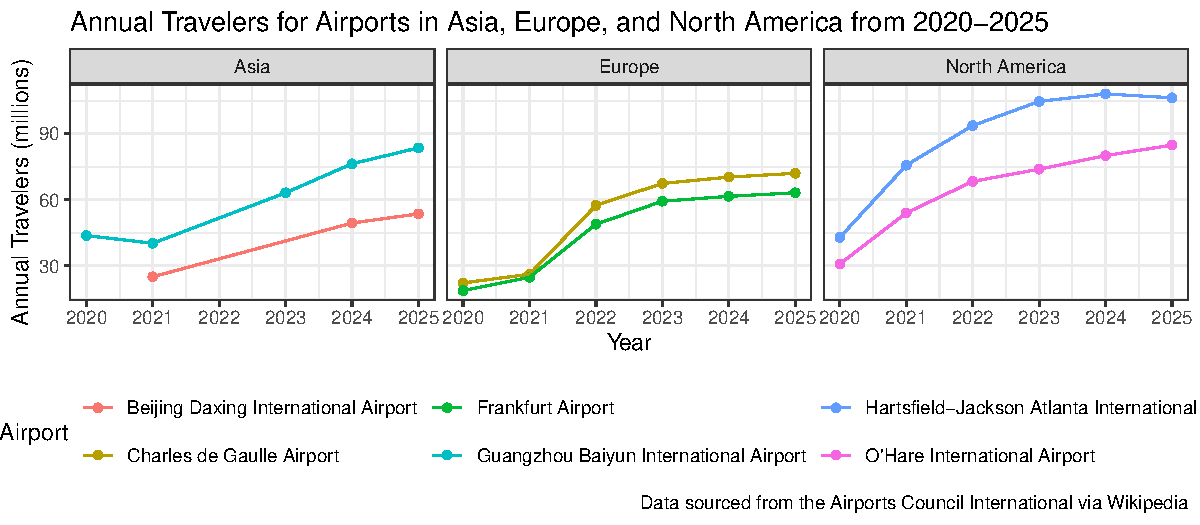
\includegraphics[keepaspectratio]{QuartoFor4.3_files/figure-pdf/fig-airportTravelers-1.pdf}}

}

\end{figure}%

Figure~\ref{fig-airportTravelers} suggests that the rapid increase in
each airport's annual travelers after the pandemic is not representative
of its future growth. The airports all saw a large increase in annual
travelers between 2021 and 2023 that has slowed growth in 2024 and 2025.
So, despite extreme maximum and minimum values, the plot suggests that
airports will see slower growth in future years as the effect of
COVID-19 lessens. Although the curves for all six airlines have similar
shapes, the airports in North America had the most pronounced rebound in
recent years, suggesting that COVID-19 may have had a larger impact on
American air travel than other nations.

\section{Monte Carlo Numerical
Integration}\label{monte-carlo-numerical-integration}

\subsection{Objective}\label{objective-1}

Monte Carlo Integration utilizes the generation of random ordered pairs
to estimate the area under a function. The main goal of this project was
to create four small multiples of 10, 100, 1,000, and 10,000 points that
integrated the probability density function for the beta distribution.
The following were all smaller-scale goals that were achieved along the
way:

\begin{enumerate}
\def\labelenumi{\arabic{enumi}.}
\tightlist
\item
  Create a function that generates a random set of ordered pairs
  depending on the user's preference of the bounds and sample size
\item
  Apply the probability beta distribution to the set of ordered pairs
  generated by the function
\item
  Create a flagging system that will show whether each ordered pair is
  above or below the output of the beta distribution function. Integrate
  the probability density function for the beta distribution based the
  number of points below the function
\item
  Create four plots that color each ordered pair based on whether it is
  above or below the function and that show the integration of the
  probability density function for the beta distribution. \#\#\# Random
  Coordinate Generator Function
\end{enumerate}

\subsection{Protocol for Monte Carlo
Integration}\label{protocol-for-monte-carlo-integration}

To use the Monte Carlo Integration method in R, you must create a random
coordinate generator function. This function must be able to take upper
and lower bounds for both x and y as parameters, as well as the sample
size that the user desires. Once this function is created, the user can
apply the beta distribution to all x-coordinates that were generated.
There must be a flagging system in place such that all y-coordinates are
labeled as being either above or below the function. This flagging
system should be implemented using both of the following methods:

\begin{enumerate}
\def\labelenumi{\arabic{enumi}.}
\tightlist
\item
  Each point should be labeled as ``above'' or ``below'' the function so
  that the points can be colored based on this attribute.
\item
  Each point should be assigned a value of 1 if it is above the function
  and a value of 0 if it is below the function.
\end{enumerate}

The second method listed above is key for estimating the area under the
curve: it allows us to easily determine what proportion of points are
below the curve (by taking the average value of this column in the
dataframe) without manually counting each point's label.

\subsection{Creating the Plots}\label{creating-the-plots}

Four plots were created: each with the x-coordinate mapped to the x-axis
and y-coordinate mapped to the y-axis. The coordinates that were
generated from the previously mentioned function are plotted on the
graph and colored based on whether they are above the curve (red) or
below it (green). The beta distribution function was also plotted for
viewers' reference. Each plot contained a different sample size of
coordinates from the coordinate generator function and listed the
estimated numerical integration below the plot (See
Figure~\ref{fig-monteCarlo}).

\begin{figure}

\caption{\label{fig-monteCarlo}Monte Carlo integration of the Beta
Distribution With Four Unique Sample Sizes}

\begin{minipage}{0.50\linewidth}

\subcaption{\label{fig-monteCarlo-1}Integration with 10 Points}

\centering{

\pandocbounded{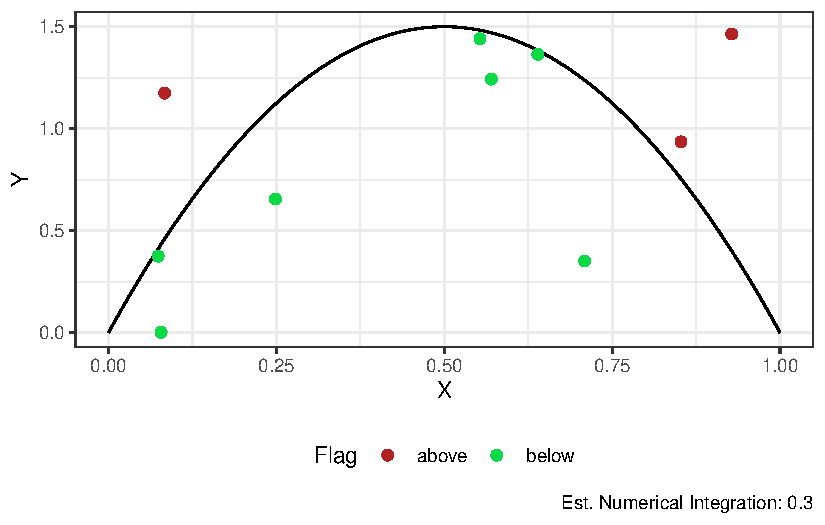
\includegraphics[keepaspectratio]{QuartoFor4.3_files/figure-pdf/fig-monteCarlo-1.pdf}}

}

\end{minipage}%
%
\begin{minipage}{0.50\linewidth}

\subcaption{\label{fig-monteCarlo-2}Integration with 100 Points}

\centering{

\pandocbounded{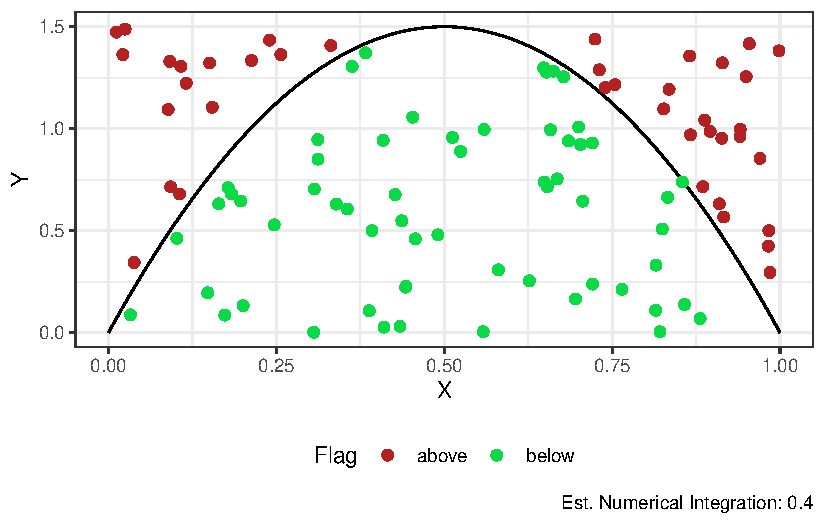
\includegraphics[keepaspectratio]{QuartoFor4.3_files/figure-pdf/fig-monteCarlo-2.pdf}}

}

\end{minipage}%
\newline
\begin{minipage}{0.50\linewidth}

\subcaption{\label{fig-monteCarlo-3}Integration with 1,000 Points}

\centering{

\pandocbounded{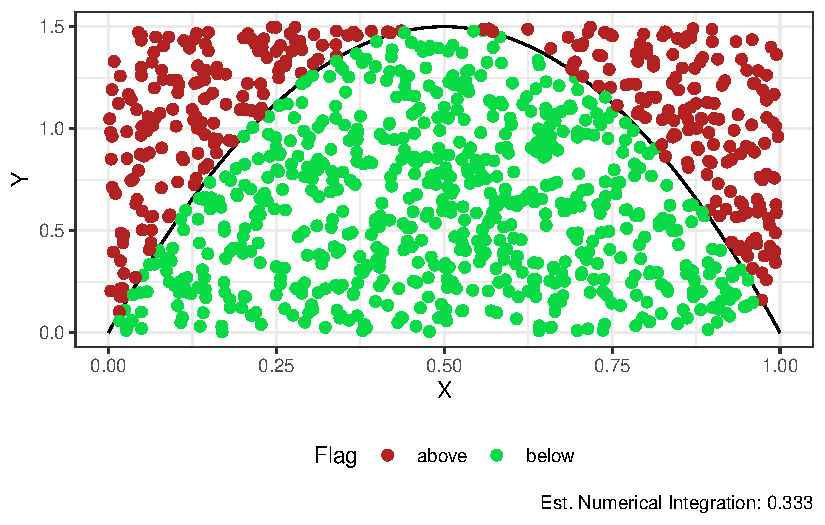
\includegraphics[keepaspectratio]{QuartoFor4.3_files/figure-pdf/fig-monteCarlo-3.pdf}}

}

\end{minipage}%
%
\begin{minipage}{0.50\linewidth}

\subcaption{\label{fig-monteCarlo-4}Integration with 10,000 Points}

\centering{

\pandocbounded{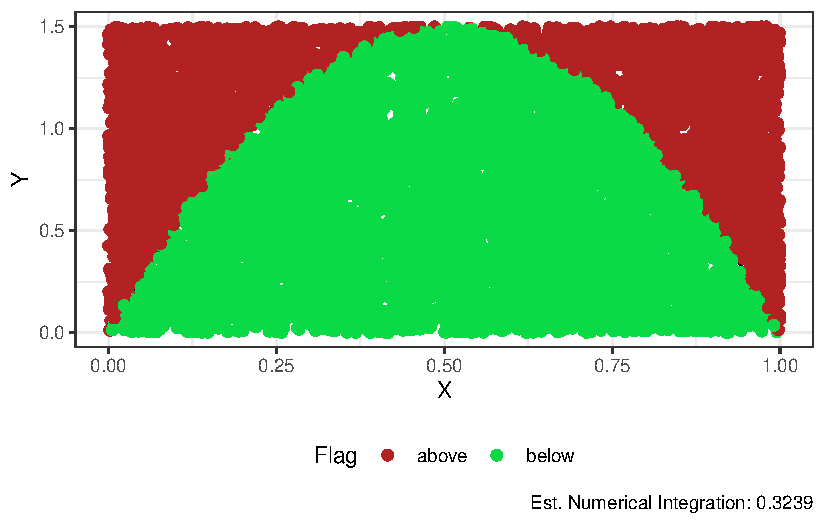
\includegraphics[keepaspectratio]{QuartoFor4.3_files/figure-pdf/fig-monteCarlo-4.pdf}}

}

\end{minipage}%

\end{figure}%

\subsection{Interpreting the Plots}\label{interpreting-the-plots}

These figures illustrate how the plotting of random ordered pairs can be
used to evaluate the area under a curve, and the area under my assigned
function is most likely 0.3363. Furthermore, the graph makes it obvious
that the estimated numerical integration becomes more precise as the
number of plotted points increases, as a larger proportion of the plot
becomes populated with coordinates. Since the estimated area depends on
whether these coordinates are flagged as above or below the curve, a
larger sample size will produce a more accurate answer for area. The
graph appeared to be full when 10,000 points were plotted, so the
corresponding estimated numerical integration of 0.3363 will match the
actual area under the curve. These small multiples suggest that if
someone else replicated this process, they would arrive at the same
conclusion as long as they plotted a sufficient number of coordinates
from the coordinate generator function.

\section{Planning and Prompting GenAI
Tools}\label{planning-and-prompting-genai-tools}

The goal of this section is to evaluate how the quality of code written
by GenAI tools differ based on the quality of the prompt they receive.
For this investigation, I focused on a study that tracked women's
calcium levels over the course of four years. Each woman was placed in
one of two treatment groups: she either participated in a regimented
diet/exercise program or did not receive any special treatment. I
provided OpenAI's ChatGPT with a detailed prompt of the relevant goals,
needs, and necessary steps to create an informative data visualization
as well as the untidied data from this experiment.

\subsection{A Detailed Plan for Data Wrangling and
Visualization}\label{a-detailed-plan-for-data-wrangling-and-visualization}

Below is the exact prompt that I provided to ChatGPT:

``Goal: To wrangle the data from the calcium csv into tidy form and
create an informative data visualization that shows how calcium levels
between both treatment groups varied over the experiment's duration

Needs:

Nouns: Plan, R Project, R Script, tidyverse, packages, calcium csv,
data, columns, scatterplot, framework, mapping, title, treatment group,
caption

Verbs: Create, Copy, Fill, Wrangle, Load, Add, Rearrange, Define, Color,
Select, Add, Render, Debug, Generate

Steps:

\begin{enumerate}
\def\labelenumi{\arabic{enumi}.}
\item
  Create my plan
\item
  Create an R Project for this work
\item
  Create a blank R script
\item
  Copy and paste the data wrangling template
\item
  Fill in the template with any relevant information
\item
  Wrangle the data

  \begin{enumerate}
  \def\labelenumii{\arabic{enumii}.}
  \item
    Load necessary packages
  \item
    Load the calcium csv file
  \item
    Add descriptive column names
  \item
    Rearrange the data so that each case is a woman in the study. The
    data in the 5th through 8th columns should be joined with the 1st
    through 4th columns so that there is one column for each year's data
  \item
    A new column should be created to identify whether the women were
    part of the null or experimental groups
  \item
    Each cell should contain the same number of decimal points
  \end{enumerate}
\item
  Create an informative data visualization that shows the difference in
  calcium levels between the null treatment and experimental groups over
  the duration of the experiment

  \begin{enumerate}
  \def\labelenumii{\arabic{enumii}.}
  \item
    Define the framework and mapping for the plot
  \item
    Color the points based on their treatment group
  \item
    Select the appropriate geometry
  \item
    Add descriptive titles for the plot axes
  \item
    Add an informative caption that cites the data source
  \item
    Render the plot
  \end{enumerate}
\item
  Debug if any errors came up
\item
  Generate Alt Text and a long description for the plot''
\end{enumerate}

\subsection{Response and Plot Generated from the Detailed
Prompt}\label{response-and-plot-generated-from-the-detailed-prompt}

When provided with a detailed prompt, ChatGPT produced a surprisingly
high-quality visual aide (See Figure~\ref{fig-chatGPTDetailedPlot}). See
the GenAI Code Appendix in Section 5.2 for its full response.

\begin{figure}[H]

\caption{\label{fig-chatGPTDetailedPlot}Graphs of annual travelers over
time for six major airports between 2020 and 2025, grouped by their
continent}

\centering{

\pandocbounded{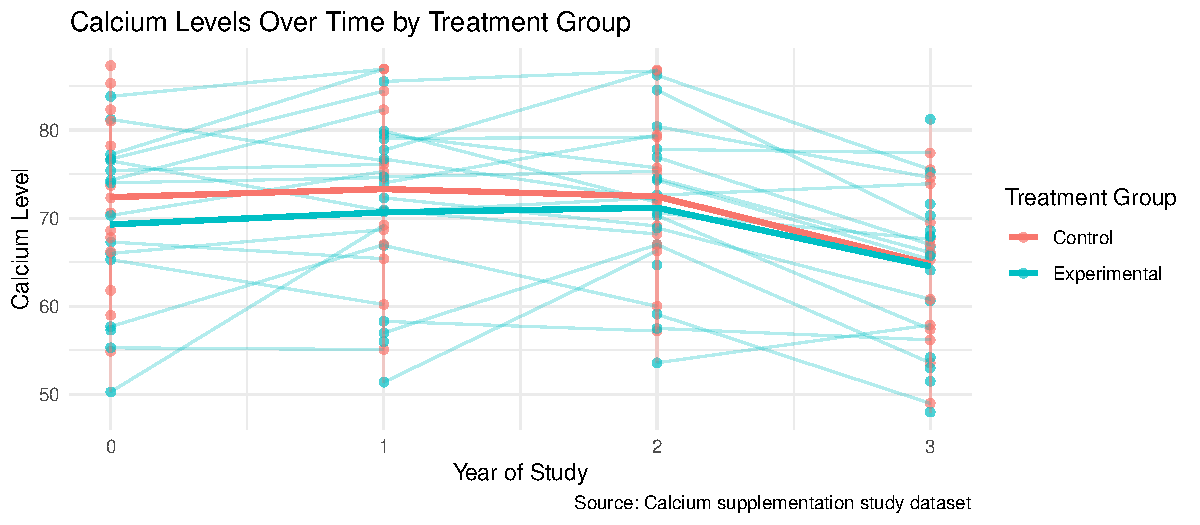
\includegraphics[keepaspectratio]{QuartoFor4.3_files/figure-pdf/fig-chatGPTDetailedPlot-1.pdf}}

}

\end{figure}%

\subsection{Response and Plot from the Generic
Prompt}\label{response-and-plot-from-the-generic-prompt}

The plot above stands in stark contrast to the data visualization
created by ChatGPT when given a generic prompt (See
Figure~\ref{fig-genericChatGPT}). The exact prompt provided was ``Create
a data visualization for these data. Calcium.csv'' See the GenAI Code
Appendix in Section 5.2 for the full generic response.

\begin{figure}

\caption{\label{fig-genericChatGPT}The line plot created by ChatGPT when
given a generic prompt}

\centering{

\pandocbounded{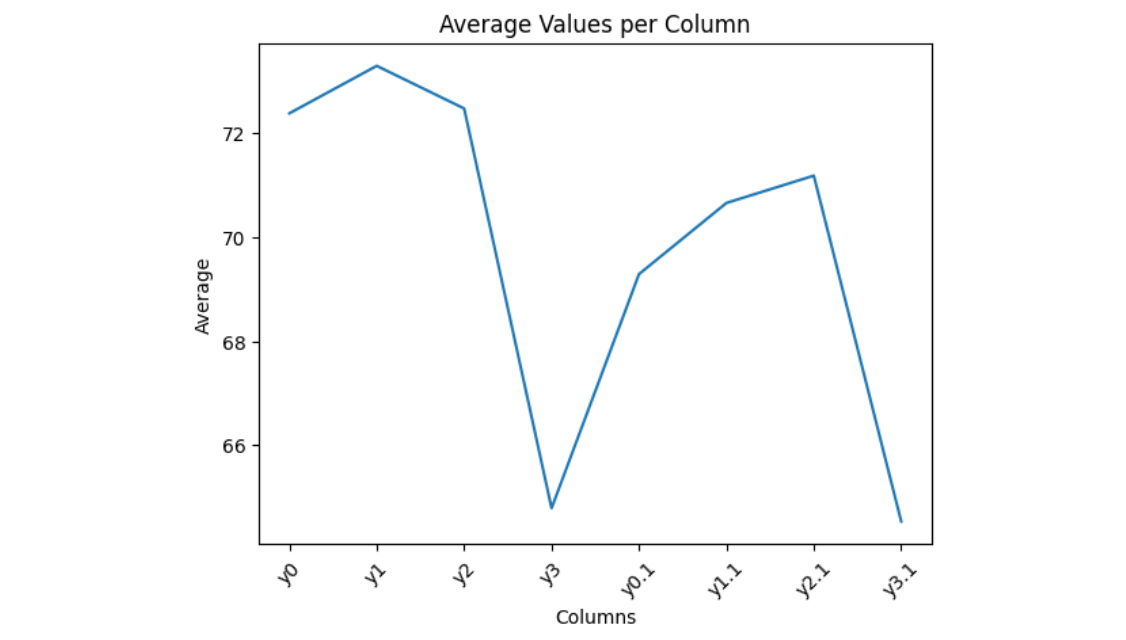
\includegraphics[keepaspectratio]{images/genericChatGPTPlot.png}}

}

\end{figure}%

\subsection{Analyzing Discrepancies in Plot Quality Between a Generic
and Detailed
Prompt}\label{analyzing-discrepancies-in-plot-quality-between-a-generic-and-detailed-prompt}

The importance of providing GenAI tools with detailed prompts can be
seen in both the text response it provided and the resulting visual.
When provided with a detailed prompt, ChatGPT addressed me as someone
with a coding background and provided me with more of an explanation
into what it was doing. However, when given a generic prompt, ChatGPT
provided a vague and unhelpful description that provided more empty
positive reinforcement than insightful information. The plots tell a
similar story: when given a detailed prompt, ChatGPT produced a
high-level plot that shows each case, distinguishes between treatment
groups, and provides the average value for each experimental group. On
the other hand, the generic prompt led it to treat all the women of each
year as a case, and it only provided the average calcium level for all
women each year. Furthermore, it failed to separate the women into two
treatment groups, which makes the plot almost entirely useless. When
working with GenAI in the future, it is crucial for myself and others to
provide clear, detailed prompts of our goals, needs, and steps. Doing so
will cause the AI technology to produce a higher-quality output and to
provide more insight into its reasoning.

\section{Reflection}\label{reflection}

\subsection{Persistence is Everything!}\label{persistence-is-everything}

When I walked into the Pollock building for the first day of my first
ever programming class, I came in with a naive view of the field. I
envisioned myself hastily typing lines of code as stunning plots and
tidy dataframes appeared on my screen. Little did I know that
(especially at first) I would receive an error message more often than
not. However, my view of those error messages transformed throughout the
course. I used to get frustrated whenever I got an error message and get
mad at both myself and R. Now, in contrast, I have found that I am
better able to roll with the punches and not the let the error messages
derail me. I had no idea how important determination and resilience
would be when learning my first programming language, and I would like
to think that I grew in both of those areas throughout the semester.

\subsection{The Importance of Being
Detail-Oriented}\label{the-importance-of-being-detail-oriented}

Another lasting impact that Stat 184 had on me is the importance of
being meticulous and detail-oriented, especially when programming. It
became clear quickly that this was a goal of the professors when we were
given the difficult task of creating a plan for making an origami paper
boat. I remember being shocked by how many steps and needs we were
supposed to have in our plan! I would like to think that the current
version of myself would be able to produce a plan that methodical and
detailed. Planning ahead is especially important in programming as the
initial time investment always proves to be worth it in the long run. I
have found that planning my code in advnance challenged me to reflect on
what I learned throughout the course and ponder the best route forward.
I am excited to apply this forward-thinking mindset to other areas of
life as well.

\newpage{}

\section{Code Appendices}\label{code-appendices}

\subsection{Personal Code Appendix}\label{personal-code-appendix}

\begin{Shaded}
\begin{Highlighting}[]
\CommentTok{\# Step 1: Load needed packages{-}{-}{-}{-}}

\FunctionTok{library}\NormalTok{(tidyverse)}
\FunctionTok{library}\NormalTok{(rvest)}
\FunctionTok{library}\NormalTok{(devtools)}
\FunctionTok{library}\NormalTok{(dcData)}
\FunctionTok{library}\NormalTok{(knitr)}
\FunctionTok{library}\NormalTok{(janitor)}
\FunctionTok{library}\NormalTok{(kableExtra)}
\FunctionTok{library}\NormalTok{(plotly)}
\CommentTok{\# Step 2: Scrape airport data{-}{-}{-}{-}}
\NormalTok{airportURL }\OtherTok{\textless{}{-}} \StringTok{"https://en.wikipedia.org/wiki/List\_of\_busiest\_airports\_by\_passenger\_traffic"}
\NormalTok{airportRawList }\OtherTok{\textless{}{-}} \FunctionTok{read\_html}\NormalTok{(}\AttributeTok{x =}\NormalTok{ airportURL) }\SpecialCharTok{|\textgreater{}}
  \FunctionTok{html\_elements}\NormalTok{(}\AttributeTok{css =} \StringTok{"table"}\NormalTok{) }\SpecialCharTok{|\textgreater{}}
  \FunctionTok{html\_table}\NormalTok{() }
\NormalTok{airportInfo2025 }\OtherTok{\textless{}{-}}\NormalTok{ airportRawList[[}\DecValTok{1}\NormalTok{]] }\SpecialCharTok{|\textgreater{}} 
  \FunctionTok{clean\_names}\NormalTok{() }\SpecialCharTok{|\textgreater{}}
  \FunctionTok{filter}\NormalTok{(}\StringTok{\textasciigrave{}}\AttributeTok{code\_iata\_icao}\StringTok{\textasciigrave{}} \SpecialCharTok{\%in\%} \FunctionTok{c}\NormalTok{(}\StringTok{"ATL/KATL"}\NormalTok{, }\StringTok{"FRA/EDDF"}\NormalTok{, }\StringTok{"PKX/ZBAD"}\NormalTok{,}
                                 \StringTok{"ORD/KORD"}\NormalTok{, }\StringTok{"CDG/LFPG"}\NormalTok{, }\StringTok{"CAN/ZGGG"}\NormalTok{)) }\SpecialCharTok{|\textgreater{}} 
  \CommentTok{\# Select only the 6 airports we are interested in}
  \FunctionTok{mutate}\NormalTok{(}\AttributeTok{year =} \DecValTok{2025}\NormalTok{) }\CommentTok{\# Add the year as an identifier}
\NormalTok{airportInfo2024 }\OtherTok{\textless{}{-}}\NormalTok{ airportRawList[[}\DecValTok{2}\NormalTok{]] }\SpecialCharTok{|\textgreater{}}
  \FunctionTok{clean\_names}\NormalTok{() }\SpecialCharTok{|\textgreater{}}
  \FunctionTok{filter}\NormalTok{(}\StringTok{\textasciigrave{}}\AttributeTok{code\_iata\_icao}\StringTok{\textasciigrave{}} \SpecialCharTok{\%in\%} \FunctionTok{c}\NormalTok{(}\StringTok{"ATL/KATL"}\NormalTok{, }\StringTok{"FRA/EDDF"}\NormalTok{, }\StringTok{"PKX/ZBAD"}\NormalTok{,}
                                 \StringTok{"ORD/KORD"}\NormalTok{, }\StringTok{"CDG/LFPG"}\NormalTok{, }\StringTok{"CAN/ZGGG"}\NormalTok{)) }\SpecialCharTok{|\textgreater{}} 
  \CommentTok{\# Select only the 6 airports we are interested in}
  \FunctionTok{mutate}\NormalTok{(}\AttributeTok{year =} \DecValTok{2024}\NormalTok{) }\CommentTok{\# Add the year as an identifier}
\NormalTok{airportInfo2023 }\OtherTok{\textless{}{-}}\NormalTok{ airportRawList[[}\DecValTok{3}\NormalTok{]] }\SpecialCharTok{|\textgreater{}}
  \FunctionTok{clean\_names}\NormalTok{() }\SpecialCharTok{|\textgreater{}}
  \FunctionTok{filter}\NormalTok{(}\StringTok{\textasciigrave{}}\AttributeTok{code\_iata\_icao}\StringTok{\textasciigrave{}} \SpecialCharTok{\%in\%} \FunctionTok{c}\NormalTok{(}\StringTok{"ATL/KATL"}\NormalTok{, }\StringTok{"FRA/EDDF"}\NormalTok{, }\StringTok{"PKX/ZBAD"}\NormalTok{,}
                                 \StringTok{"ORD/KORD"}\NormalTok{, }\StringTok{"CDG/LFPG"}\NormalTok{, }\StringTok{"CAN/ZGGG"}\NormalTok{)) }\SpecialCharTok{|\textgreater{}} 
  \CommentTok{\# Select only the 6 airports we are interested in}
  \FunctionTok{mutate}\NormalTok{(}\AttributeTok{year =} \DecValTok{2023}\NormalTok{) }\CommentTok{\# Add the year as an identifier}
\NormalTok{airportInfo2022 }\OtherTok{\textless{}{-}}\NormalTok{ airportRawList[[}\DecValTok{4}\NormalTok{]] }\SpecialCharTok{|\textgreater{}}
  \FunctionTok{clean\_names}\NormalTok{() }\SpecialCharTok{|\textgreater{}}
  \FunctionTok{filter}\NormalTok{(}\StringTok{\textasciigrave{}}\AttributeTok{code\_iata\_icao}\StringTok{\textasciigrave{}} \SpecialCharTok{\%in\%} \FunctionTok{c}\NormalTok{(}\StringTok{"ATL/KATL"}\NormalTok{, }\StringTok{"FRA/EDDF"}\NormalTok{, }\StringTok{"PKX/ZBAD"}\NormalTok{,}
                                 \StringTok{"ORD/KORD"}\NormalTok{, }\StringTok{"CDG/LFPG"}\NormalTok{, }\StringTok{"CAN/ZGGG"}\NormalTok{)) }\SpecialCharTok{|\textgreater{}} 
  \CommentTok{\# Select only the 6 airports we are interested in}
  \FunctionTok{mutate}\NormalTok{(}\AttributeTok{year =} \DecValTok{2022}\NormalTok{) }\CommentTok{\# Add the year as an identifier}
\NormalTok{airportInfo2021 }\OtherTok{\textless{}{-}}\NormalTok{ airportRawList[[}\DecValTok{5}\NormalTok{]] }\SpecialCharTok{|\textgreater{}}
  \FunctionTok{clean\_names}\NormalTok{() }\SpecialCharTok{|\textgreater{}}
  \FunctionTok{filter}\NormalTok{(}\StringTok{\textasciigrave{}}\AttributeTok{code\_iata\_icao}\StringTok{\textasciigrave{}} \SpecialCharTok{\%in\%} \FunctionTok{c}\NormalTok{(}\StringTok{"ATL/KATL"}\NormalTok{, }\StringTok{"FRA/EDDF"}\NormalTok{, }\StringTok{"PKX/ZBAD"}\NormalTok{,}
                                 \StringTok{"ORD/KORD"}\NormalTok{, }\StringTok{"CDG/LFPG"}\NormalTok{, }\StringTok{"CAN/ZGGG"}\NormalTok{)) }\SpecialCharTok{|\textgreater{}} 
  \CommentTok{\# Select only the 6 airports we are interested in}
  \FunctionTok{mutate}\NormalTok{(}\AttributeTok{year =} \DecValTok{2021}\NormalTok{) }\CommentTok{\# Add the year as an identifier}
\NormalTok{airportInfo2020 }\OtherTok{\textless{}{-}}\NormalTok{ airportRawList[[}\DecValTok{6}\NormalTok{]] }\SpecialCharTok{|\textgreater{}}
  \FunctionTok{clean\_names}\NormalTok{() }\SpecialCharTok{|\textgreater{}}
  \FunctionTok{filter}\NormalTok{(}\StringTok{\textasciigrave{}}\AttributeTok{code\_iata\_icao}\StringTok{\textasciigrave{}} \SpecialCharTok{\%in\%} \FunctionTok{c}\NormalTok{(}\StringTok{"ATL/KATL"}\NormalTok{, }\StringTok{"FRA/EDDF"}\NormalTok{, }\StringTok{"PKX/ZBAD"}\NormalTok{,}
                                 \StringTok{"ORD/KORD"}\NormalTok{, }\StringTok{"CDG/LFPG"}\NormalTok{, }\StringTok{"CAN/ZGGG"}\NormalTok{)) }\SpecialCharTok{|\textgreater{}} 
  \CommentTok{\# Select only the 6 airports we are interested in}
  \FunctionTok{mutate}\NormalTok{(}\AttributeTok{year =} \DecValTok{2020}\NormalTok{) }\CommentTok{\# Add the year as an identifier}
  
\CommentTok{\#Step 3: Wrangle and join the dataframes{-}{-}{-}{-}}

\NormalTok{airportProgress }\OtherTok{\textless{}{-}} \FunctionTok{bind\_rows}\NormalTok{(airportInfo2025, airportInfo2024,}
\NormalTok{                             airportInfo2023, airportInfo2022, airportInfo2021, airportInfo2020) }\SpecialCharTok{|\textgreater{}} 
  \CommentTok{\# Join the dataframes so that each case is an airport and year }
  \FunctionTok{separate\_wider\_delim}\NormalTok{( }
    \AttributeTok{cols =}\NormalTok{ totalpassengers, }\CommentTok{\# Separate the numerical value from the text in brackets}
    \AttributeTok{delim =} \StringTok{"["}\NormalTok{,}
    \AttributeTok{names =} \FunctionTok{c}\NormalTok{(}\StringTok{"annualTravelers"}\NormalTok{, }\StringTok{"unnecessaryInfo"}\NormalTok{),}
    \AttributeTok{too\_few =} \StringTok{"align\_start"}\NormalTok{,}
    \AttributeTok{too\_many =} \StringTok{"merge"}
\NormalTok{  ) }\SpecialCharTok{|\textgreater{}}
  \FunctionTok{select}\NormalTok{(}\SpecialCharTok{{-}}\NormalTok{unnecessaryInfo) }\SpecialCharTok{|\textgreater{}} \CommentTok{\# Remove the column containing the unnecessary text in brackets}
  \FunctionTok{rename}\NormalTok{(}
    \StringTok{"annual\%Change"} \OtherTok{=} \StringTok{"percent\_change"} \CommentTok{\# Add a descriptive column name}
\NormalTok{  ) }\SpecialCharTok{|\textgreater{}}
  \FunctionTok{separate\_wider\_delim}\NormalTok{( }\CommentTok{\# Isolate the percent symbol from the numerical entry}
    \AttributeTok{cols =} \StringTok{"annual\%Change"}\NormalTok{,}
    \AttributeTok{delim =} \StringTok{"\%"}\NormalTok{,}
    \AttributeTok{names =} \FunctionTok{c}\NormalTok{(}\StringTok{"annualPercentChange"}\NormalTok{, }\StringTok{"Junk"}\NormalTok{)) }\SpecialCharTok{|\textgreater{}}
  \FunctionTok{select}\NormalTok{(}\SpecialCharTok{{-}}\NormalTok{Junk, }\SpecialCharTok{{-}}\NormalTok{rank) }\SpecialCharTok{|\textgreater{}} \CommentTok{\# Remove the percent symbols and the Rank column}
  \FunctionTok{mutate}\NormalTok{(}
    \AttributeTok{annualTravelers =} \FunctionTok{parse\_number}\NormalTok{(annualTravelers), }
    \CommentTok{\# Remove the commas from cells}
    \AttributeTok{annualPercentChange =} \FunctionTok{as.numeric}\NormalTok{(annualPercentChange), }
    \CommentTok{\# Pass the contents in this column as numeric, not character strings}
    \AttributeTok{annualPercentChange =} \FunctionTok{case\_when}\NormalTok{( }
      \CommentTok{\# Add back the negative signs that got dropped during data scraping }
\NormalTok{      annualPercentChange }\SpecialCharTok{==} \FloatTok{01.6} \SpecialCharTok{\textasciitilde{}} \SpecialCharTok{{-}}\FloatTok{01.6}\NormalTok{,}
\NormalTok{      annualPercentChange }\SpecialCharTok{==} \FloatTok{8.0} \SpecialCharTok{\textasciitilde{}} \SpecialCharTok{{-}}\FloatTok{8.0}\NormalTok{,}
\NormalTok{      annualPercentChange }\SpecialCharTok{==} \FloatTok{40.4} \SpecialCharTok{\textasciitilde{}} \SpecialCharTok{{-}}\FloatTok{40.4}\NormalTok{,}
\NormalTok{      annualPercentChange }\SpecialCharTok{==} \FloatTok{61.2} \SpecialCharTok{\textasciitilde{}} \SpecialCharTok{{-}}\FloatTok{61.2}\NormalTok{,}
\NormalTok{      annualPercentChange }\SpecialCharTok{==} \FloatTok{63.5} \SpecialCharTok{\textasciitilde{}} \SpecialCharTok{{-}}\FloatTok{63.5}\NormalTok{,}
\NormalTok{      annualPercentChange }\SpecialCharTok{==} \FloatTok{70.8} \SpecialCharTok{\textasciitilde{}} \SpecialCharTok{{-}}\FloatTok{70.8}\NormalTok{,}
\NormalTok{      annualPercentChange }\SpecialCharTok{==} \FloatTok{73.4} \SpecialCharTok{\textasciitilde{}} \SpecialCharTok{{-}}\FloatTok{73.4}\NormalTok{,}
      \AttributeTok{.default =}\NormalTok{ annualPercentChange)) }\SpecialCharTok{|\textgreater{}}
  \FunctionTok{rename}\NormalTok{(}\AttributeTok{annualRankChange =}\NormalTok{ rankchange) }\SpecialCharTok{|\textgreater{}} 
  \CommentTok{\# Create a more descriptive column name}
  \FunctionTok{mutate}\NormalTok{(}
    \AttributeTok{annualRankChange =} \FunctionTok{replace\_na}\NormalTok{(annualRankChange, }\DecValTok{0}\NormalTok{,), }
    \CommentTok{\# Replace NA values with 0}
    \AttributeTok{continent =} \FunctionTok{case\_when}\NormalTok{( }\CommentTok{\# Add a column containing each airport\textquotesingle{}s continent}
\NormalTok{      country }\SpecialCharTok{==} \StringTok{"United States"} \SpecialCharTok{\textasciitilde{}} \StringTok{"North America"}\NormalTok{,}
\NormalTok{      country }\SpecialCharTok{==} \StringTok{"China"} \SpecialCharTok{\textasciitilde{}} \StringTok{"Asia"}\NormalTok{,}
\NormalTok{      country }\SpecialCharTok{==} \StringTok{"France"} \SpecialCharTok{\textasciitilde{}} \StringTok{"Europe"}\NormalTok{,}
\NormalTok{      country }\SpecialCharTok{==} \StringTok{"Germany"} \SpecialCharTok{\textasciitilde{}} \StringTok{"Europe"}
\NormalTok{    )}
\NormalTok{  )}

\NormalTok{airportPercentChange }\OtherTok{\textless{}{-}}\NormalTok{ airportProgress }\SpecialCharTok{|\textgreater{}}
  \FunctionTok{group\_by}\NormalTok{(airport) }\SpecialCharTok{|\textgreater{}}
  \FunctionTok{summarise}\NormalTok{(}\CommentTok{\# Compute minimum percent change}
            \AttributeTok{minAnnualPercentChange =} \FunctionTok{min}\NormalTok{(annualPercentChange, }\AttributeTok{na.rm =} \ConstantTok{TRUE}\NormalTok{), }
            \CommentTok{\# Compute maximum percent change}
            \AttributeTok{maxAnnualPercentChange =} \FunctionTok{max}\NormalTok{(annualPercentChange, }\AttributeTok{na.rm =} \ConstantTok{TRUE}\NormalTok{), }
            \CommentTok{\# Compute average percent change}
            \AttributeTok{avgAnnualPercentChange =} \FunctionTok{mean}\NormalTok{(annualPercentChange, }\AttributeTok{na.rm =} \ConstantTok{TRUE}\NormalTok{), }
            \CommentTok{\# Compute median percent change}
            \AttributeTok{medianAnnualPercentChange =} \FunctionTok{median}\NormalTok{(annualPercentChange, }\AttributeTok{na.rm =} \ConstantTok{TRUE}\NormalTok{), }
            \CommentTok{\# Compute st dev for percent change}
            \AttributeTok{stdevAnnualPercentChange =} \FunctionTok{sd}\NormalTok{(annualPercentChange, }\AttributeTok{na.rm =} \ConstantTok{TRUE}\NormalTok{), }
\NormalTok{            )}
\NormalTok{airportPercentChange }\SpecialCharTok{|\textgreater{}}
\NormalTok{  knitr}\SpecialCharTok{::}\FunctionTok{kable}\NormalTok{(}
    \AttributeTok{format =} \StringTok{"latex"}\NormalTok{,}
    \AttributeTok{digits =} \DecValTok{2}\NormalTok{, }\CommentTok{\# Truncate values to two decimal places}
    \AttributeTok{format.args =} \FunctionTok{list}\NormalTok{(}\AttributeTok{big.mark =} \StringTok{\textquotesingle{},\textquotesingle{}}\NormalTok{), }\CommentTok{\# Add commas where necessary}
    \AttributeTok{align =} \StringTok{\textquotesingle{}lccccc\textquotesingle{}}\NormalTok{, }\CommentTok{\# Align the text}
    \AttributeTok{col.names =} \FunctionTok{c}\NormalTok{(}\StringTok{\textquotesingle{}Airport\textquotesingle{}}\NormalTok{, }\StringTok{\textquotesingle{}Min Annual Percent Change\textquotesingle{}}\NormalTok{, }
                  \StringTok{\textquotesingle{}Max Annual Percent Change\textquotesingle{}}\NormalTok{, }
                  \StringTok{\textquotesingle{}Average Annual Percent Change\textquotesingle{}}\NormalTok{, }
                  \StringTok{\textquotesingle{}Median Annual Percent Change\textquotesingle{}}\NormalTok{, }
                  \StringTok{\textquotesingle{}St Dev Annual Percent Change\textquotesingle{}}\NormalTok{) }
    \CommentTok{\# Add descriptive column names}
\NormalTok{  ) }\SpecialCharTok{|\textgreater{}}
  \FunctionTok{kable\_classic}\NormalTok{(}
    \AttributeTok{lightable\_options =} \StringTok{\textquotesingle{}striped\textquotesingle{}} 
    \CommentTok{\# Added light stripes to make the table more visually appealling}
\NormalTok{  ) }\SpecialCharTok{|\textgreater{}}
  \FunctionTok{footnote}\NormalTok{( }\CommentTok{\# Add a footnote describing the data source}
    \AttributeTok{general =} \StringTok{\textquotesingle{}Data sourced from the Airports Council International via Wikipedia\textquotesingle{}}\NormalTok{,}
    \AttributeTok{footnote\_as\_chunk =} \ConstantTok{TRUE} \CommentTok{\# Fit the format on one line}
\NormalTok{  ) }\SpecialCharTok{|\textgreater{}}
\NormalTok{    kableExtra}\SpecialCharTok{::}\FunctionTok{kable\_styling}\NormalTok{(}\AttributeTok{latex\_options =} \StringTok{"scale\_down"}\NormalTok{)}

\CommentTok{\# Step 1: Load needed packages{-}{-}{-}{-}}

\FunctionTok{library}\NormalTok{(tidyverse)}
\FunctionTok{library}\NormalTok{(rvest)}
\FunctionTok{library}\NormalTok{(devtools)}
\FunctionTok{library}\NormalTok{(dcData)}
\FunctionTok{library}\NormalTok{(knitr)}
\FunctionTok{library}\NormalTok{(janitor)}
\FunctionTok{library}\NormalTok{(kableExtra)}
\FunctionTok{library}\NormalTok{(plotly)}
\CommentTok{\# Step 2: Scrape airport data{-}{-}{-}{-}}
\NormalTok{airportURL }\OtherTok{\textless{}{-}} \StringTok{"https://en.wikipedia.org/wiki/List\_of\_busiest\_airports\_by\_passenger\_traffic"}
\NormalTok{airportRawList }\OtherTok{\textless{}{-}} \FunctionTok{read\_html}\NormalTok{(}\AttributeTok{x =}\NormalTok{ airportURL) }\SpecialCharTok{|\textgreater{}}
  \FunctionTok{html\_elements}\NormalTok{(}\AttributeTok{css =} \StringTok{"table"}\NormalTok{) }\SpecialCharTok{|\textgreater{}}
  \FunctionTok{html\_table}\NormalTok{() }
\NormalTok{airportInfo2025 }\OtherTok{\textless{}{-}}\NormalTok{ airportRawList[[}\DecValTok{1}\NormalTok{]] }\SpecialCharTok{|\textgreater{}} 
  \FunctionTok{clean\_names}\NormalTok{() }\SpecialCharTok{|\textgreater{}}
  \FunctionTok{filter}\NormalTok{(}\StringTok{\textasciigrave{}}\AttributeTok{code\_iata\_icao}\StringTok{\textasciigrave{}} \SpecialCharTok{\%in\%} \FunctionTok{c}\NormalTok{(}\StringTok{"ATL/KATL"}\NormalTok{, }\StringTok{"FRA/EDDF"}\NormalTok{, }\StringTok{"PKX/ZBAD"}\NormalTok{,}
                                 \StringTok{"ORD/KORD"}\NormalTok{, }\StringTok{"CDG/LFPG"}\NormalTok{, }\StringTok{"CAN/ZGGG"}\NormalTok{)) }\SpecialCharTok{|\textgreater{}} 
  \CommentTok{\# Select only the 6 airports we are interested in}
  \FunctionTok{mutate}\NormalTok{(}\AttributeTok{year =} \DecValTok{2025}\NormalTok{) }\CommentTok{\# Add the year as an identifier}
\NormalTok{airportInfo2024 }\OtherTok{\textless{}{-}}\NormalTok{ airportRawList[[}\DecValTok{2}\NormalTok{]] }\SpecialCharTok{|\textgreater{}}
  \FunctionTok{clean\_names}\NormalTok{() }\SpecialCharTok{|\textgreater{}}
  \FunctionTok{filter}\NormalTok{(}\StringTok{\textasciigrave{}}\AttributeTok{code\_iata\_icao}\StringTok{\textasciigrave{}} \SpecialCharTok{\%in\%} \FunctionTok{c}\NormalTok{(}\StringTok{"ATL/KATL"}\NormalTok{, }\StringTok{"FRA/EDDF"}\NormalTok{, }\StringTok{"PKX/ZBAD"}\NormalTok{, }
                                 \StringTok{"ORD/KORD"}\NormalTok{, }\StringTok{"CDG/LFPG"}\NormalTok{, }\StringTok{"CAN/ZGGG"}\NormalTok{)) }\SpecialCharTok{|\textgreater{}} 
  \CommentTok{\# Select only the 6 airports we are interested in}
  \FunctionTok{mutate}\NormalTok{(}\AttributeTok{year =} \DecValTok{2024}\NormalTok{) }\CommentTok{\# Add the year as an identifier}
\NormalTok{airportInfo2023 }\OtherTok{\textless{}{-}}\NormalTok{ airportRawList[[}\DecValTok{3}\NormalTok{]] }\SpecialCharTok{|\textgreater{}}
  \FunctionTok{clean\_names}\NormalTok{() }\SpecialCharTok{|\textgreater{}}
  \FunctionTok{filter}\NormalTok{(}\StringTok{\textasciigrave{}}\AttributeTok{code\_iata\_icao}\StringTok{\textasciigrave{}} \SpecialCharTok{\%in\%} \FunctionTok{c}\NormalTok{(}\StringTok{"ATL/KATL"}\NormalTok{, }\StringTok{"FRA/EDDF"}\NormalTok{, }\StringTok{"PKX/ZBAD"}\NormalTok{, }
                                 \StringTok{"ORD/KORD"}\NormalTok{, }\StringTok{"CDG/LFPG"}\NormalTok{, }\StringTok{"CAN/ZGGG"}\NormalTok{)) }\SpecialCharTok{|\textgreater{}} 
  \CommentTok{\# Select only the 6 airports we are interested in}
  \FunctionTok{mutate}\NormalTok{(}\AttributeTok{year =} \DecValTok{2023}\NormalTok{) }\CommentTok{\# Add the year as an identifier}
\NormalTok{airportInfo2022 }\OtherTok{\textless{}{-}}\NormalTok{ airportRawList[[}\DecValTok{4}\NormalTok{]] }\SpecialCharTok{|\textgreater{}}
  \FunctionTok{clean\_names}\NormalTok{() }\SpecialCharTok{|\textgreater{}}
  \FunctionTok{filter}\NormalTok{(}\StringTok{\textasciigrave{}}\AttributeTok{code\_iata\_icao}\StringTok{\textasciigrave{}} \SpecialCharTok{\%in\%} \FunctionTok{c}\NormalTok{(}\StringTok{"ATL/KATL"}\NormalTok{, }\StringTok{"FRA/EDDF"}\NormalTok{, }\StringTok{"PKX/ZBAD"}\NormalTok{, }
                                 \StringTok{"ORD/KORD"}\NormalTok{, }\StringTok{"CDG/LFPG"}\NormalTok{, }\StringTok{"CAN/ZGGG"}\NormalTok{)) }\SpecialCharTok{|\textgreater{}} 
  \CommentTok{\# Select only the 6 airports we are interested in}
  \FunctionTok{mutate}\NormalTok{(}\AttributeTok{year =} \DecValTok{2022}\NormalTok{) }\CommentTok{\# Add the year as an identifier}
\NormalTok{airportInfo2021 }\OtherTok{\textless{}{-}}\NormalTok{ airportRawList[[}\DecValTok{5}\NormalTok{]] }\SpecialCharTok{|\textgreater{}}
  \FunctionTok{clean\_names}\NormalTok{() }\SpecialCharTok{|\textgreater{}}
  \FunctionTok{filter}\NormalTok{(}\StringTok{\textasciigrave{}}\AttributeTok{code\_iata\_icao}\StringTok{\textasciigrave{}} \SpecialCharTok{\%in\%} \FunctionTok{c}\NormalTok{(}\StringTok{"ATL/KATL"}\NormalTok{, }\StringTok{"FRA/EDDF"}\NormalTok{, }\StringTok{"PKX/ZBAD"}\NormalTok{, }
                                 \StringTok{"ORD/KORD"}\NormalTok{, }\StringTok{"CDG/LFPG"}\NormalTok{, }\StringTok{"CAN/ZGGG"}\NormalTok{)) }\SpecialCharTok{|\textgreater{}} 
  \CommentTok{\# Select only the 6 airports we are interested in}
  \FunctionTok{mutate}\NormalTok{(}\AttributeTok{year =} \DecValTok{2021}\NormalTok{) }\CommentTok{\# Add the year as an identifier}
\NormalTok{airportInfo2020 }\OtherTok{\textless{}{-}}\NormalTok{ airportRawList[[}\DecValTok{6}\NormalTok{]] }\SpecialCharTok{|\textgreater{}}
  \FunctionTok{clean\_names}\NormalTok{() }\SpecialCharTok{|\textgreater{}}
  \FunctionTok{filter}\NormalTok{(}\StringTok{\textasciigrave{}}\AttributeTok{code\_iata\_icao}\StringTok{\textasciigrave{}} \SpecialCharTok{\%in\%} \FunctionTok{c}\NormalTok{(}\StringTok{"ATL/KATL"}\NormalTok{, }\StringTok{"FRA/EDDF"}\NormalTok{, }\StringTok{"PKX/ZBAD"}\NormalTok{, }
                                 \StringTok{"ORD/KORD"}\NormalTok{, }\StringTok{"CDG/LFPG"}\NormalTok{, }\StringTok{"CAN/ZGGG"}\NormalTok{)) }\SpecialCharTok{|\textgreater{}} 
  \CommentTok{\# Select only the 6 airports we are interested in}
  \FunctionTok{mutate}\NormalTok{(}\AttributeTok{year =} \DecValTok{2020}\NormalTok{) }\CommentTok{\# Add the year as an identifier}
  
\CommentTok{\#Step 3: Wrangle and join the dataframes{-}{-}{-}{-}}

\NormalTok{airportProgress }\OtherTok{\textless{}{-}} \FunctionTok{bind\_rows}\NormalTok{(airportInfo2025, airportInfo2024, }
\NormalTok{                             airportInfo2023, airportInfo2022, airportInfo2021, airportInfo2020) }\SpecialCharTok{|\textgreater{}} \CommentTok{\# Join the dataframes so that each case is an airport and year }
  \FunctionTok{separate\_wider\_delim}\NormalTok{( }
    \AttributeTok{cols =}\NormalTok{ totalpassengers, }\CommentTok{\# Isolate the numerical value }
    \AttributeTok{delim =} \StringTok{"["}\NormalTok{,}
    \AttributeTok{names =} \FunctionTok{c}\NormalTok{(}\StringTok{"annualTravelers"}\NormalTok{, }\StringTok{"unnecessaryInfo"}\NormalTok{),}
    \AttributeTok{too\_few =} \StringTok{"align\_start"}\NormalTok{,}
    \AttributeTok{too\_many =} \StringTok{"merge"}
\NormalTok{  ) }\SpecialCharTok{|\textgreater{}}
  \FunctionTok{select}\NormalTok{(}\SpecialCharTok{{-}}\NormalTok{unnecessaryInfo) }\SpecialCharTok{|\textgreater{}} \CommentTok{\# Remove unnecessary text}
  \FunctionTok{rename}\NormalTok{(}
    \StringTok{"annual\%Change"} \OtherTok{=} \StringTok{"percent\_change"} \CommentTok{\# Add a descriptive column name}
\NormalTok{  ) }\SpecialCharTok{|\textgreater{}}
  \FunctionTok{separate\_wider\_delim}\NormalTok{( }\CommentTok{\# Isolate the percent symbol from the numerical entry}
    \AttributeTok{cols =} \StringTok{"annual\%Change"}\NormalTok{,}
    \AttributeTok{delim =} \StringTok{"\%"}\NormalTok{,}
    \AttributeTok{names =} \FunctionTok{c}\NormalTok{(}\StringTok{"annualPercentChange"}\NormalTok{, }\StringTok{"Junk"}\NormalTok{)) }\SpecialCharTok{|\textgreater{}}
  \FunctionTok{select}\NormalTok{(}\SpecialCharTok{{-}}\NormalTok{Junk, }\SpecialCharTok{{-}}\NormalTok{rank) }\SpecialCharTok{|\textgreater{}} \CommentTok{\# Remove the percent symbols and the Rank column}
  \FunctionTok{mutate}\NormalTok{(}
    \AttributeTok{annualTravelers =} \FunctionTok{parse\_number}\NormalTok{(annualTravelers),}
    \CommentTok{\# Removed the commas from cells}
    \AttributeTok{annualPercentChange =} \FunctionTok{as.numeric}\NormalTok{(annualPercentChange), }
    \CommentTok{\# Passed the contents in this column as numeric, not character strings}
    \AttributeTok{annualPercentChange =} \FunctionTok{case\_when}\NormalTok{( }
      \CommentTok{\# Added back the negative signs that got dropped during data scraping }
\NormalTok{      annualPercentChange }\SpecialCharTok{==} \FloatTok{01.6} \SpecialCharTok{\textasciitilde{}} \SpecialCharTok{{-}}\FloatTok{01.6}\NormalTok{,}
\NormalTok{      annualPercentChange }\SpecialCharTok{==} \FloatTok{8.0} \SpecialCharTok{\textasciitilde{}} \SpecialCharTok{{-}}\FloatTok{8.0}\NormalTok{,}
\NormalTok{      annualPercentChange }\SpecialCharTok{==} \FloatTok{40.4} \SpecialCharTok{\textasciitilde{}} \SpecialCharTok{{-}}\FloatTok{40.4}\NormalTok{,}
\NormalTok{      annualPercentChange }\SpecialCharTok{==} \FloatTok{61.2} \SpecialCharTok{\textasciitilde{}} \SpecialCharTok{{-}}\FloatTok{61.2}\NormalTok{,}
\NormalTok{      annualPercentChange }\SpecialCharTok{==} \FloatTok{63.5} \SpecialCharTok{\textasciitilde{}} \SpecialCharTok{{-}}\FloatTok{63.5}\NormalTok{,}
\NormalTok{      annualPercentChange }\SpecialCharTok{==} \FloatTok{70.8} \SpecialCharTok{\textasciitilde{}} \SpecialCharTok{{-}}\FloatTok{70.8}\NormalTok{,}
\NormalTok{      annualPercentChange }\SpecialCharTok{==} \FloatTok{73.4} \SpecialCharTok{\textasciitilde{}} \SpecialCharTok{{-}}\FloatTok{73.4}\NormalTok{,}
      \AttributeTok{.default =}\NormalTok{ annualPercentChange)) }\SpecialCharTok{|\textgreater{}}
  \FunctionTok{rename}\NormalTok{(}\AttributeTok{annualRankChange =}\NormalTok{ rankchange) }\SpecialCharTok{|\textgreater{}} 
  \CommentTok{\# Created a more descriptive column name}
  \FunctionTok{mutate}\NormalTok{(}
    \AttributeTok{annualRankChange =} \FunctionTok{replace\_na}\NormalTok{(annualRankChange, }\DecValTok{0}\NormalTok{,), }\CommentTok{\# Replace NA values with 0}
    \AttributeTok{continent =} \FunctionTok{case\_when}\NormalTok{( }\CommentTok{\# Add a column containing each airport\textquotesingle{}s continent }
\NormalTok{      country }\SpecialCharTok{==} \StringTok{"United States"} \SpecialCharTok{\textasciitilde{}} \StringTok{"North America"}\NormalTok{,}
\NormalTok{      country }\SpecialCharTok{==} \StringTok{"China"} \SpecialCharTok{\textasciitilde{}} \StringTok{"Asia"}\NormalTok{,}
\NormalTok{      country }\SpecialCharTok{==} \StringTok{"France"} \SpecialCharTok{\textasciitilde{}} \StringTok{"Europe"}\NormalTok{,}
\NormalTok{      country }\SpecialCharTok{==} \StringTok{"Germany"} \SpecialCharTok{\textasciitilde{}} \StringTok{"Europe"}
\NormalTok{    )}
\NormalTok{  )}

\NormalTok{airportPlotData }\OtherTok{\textless{}{-}}\NormalTok{ airportProgress }\SpecialCharTok{|\textgreater{}}
  \FunctionTok{mutate}\NormalTok{(}\AttributeTok{annualTravelers =}\NormalTok{ annualTravelers }\SpecialCharTok{/} \DecValTok{1000000}\NormalTok{)}

\FunctionTok{ggplot}\NormalTok{( }\CommentTok{\# Create the plot\textquotesingle{}s frame}
  \AttributeTok{data =}\NormalTok{ airportPlotData,}
  \AttributeTok{mapping =} \FunctionTok{aes}\NormalTok{( }\CommentTok{\# map year to the x{-}axis and annual travelers to the y{-}axis}
    \AttributeTok{x =}\NormalTok{ year,}
    \AttributeTok{y =}\NormalTok{ annualTravelers,}
    \AttributeTok{color =}\NormalTok{ airport, }\CommentTok{\# Color points based on their Airport name}
\NormalTok{  )}
\NormalTok{) }\SpecialCharTok{+}
  \FunctionTok{geom\_point}\NormalTok{() }\SpecialCharTok{+} \CommentTok{\# Create a scatterplot}
  \FunctionTok{geom\_line}\NormalTok{() }\SpecialCharTok{+} \CommentTok{\# Improvement: Connect the points for each airport}
  \FunctionTok{scale\_color\_hue}\NormalTok{(}\AttributeTok{direction =} \DecValTok{1}\NormalTok{) }\SpecialCharTok{+}
  \FunctionTok{labs}\NormalTok{( }\CommentTok{\# Improvement: Add descriptive axis titles, labels, and a plot title}
    \AttributeTok{x =} \StringTok{"Year"}\NormalTok{,}
    \AttributeTok{y =} \StringTok{"Annual Travelers (millions)"}\NormalTok{,}
    \AttributeTok{color =} \StringTok{"Airport"}\NormalTok{,}
    \AttributeTok{title =} \StringTok{"Annual Travelers for Airports in Asia, Europe, and North America from 2020{-}2025"}\NormalTok{,}
    \AttributeTok{caption =} \StringTok{"Data sourced from the Airports Council International via Wikipedia"}\NormalTok{) }\SpecialCharTok{+}
  \FunctionTok{facet\_wrap}\NormalTok{(}\SpecialCharTok{\textasciitilde{}}\NormalTok{ continent) }\SpecialCharTok{+} \CommentTok{\# Create three facets: one for each continent }
  \FunctionTok{theme\_bw}\NormalTok{() }\SpecialCharTok{+} \CommentTok{\# Select the black and white background for visual appeal}
  \FunctionTok{theme}\NormalTok{(}
    \AttributeTok{legend.position =} \StringTok{"bottom"} \CommentTok{\# Align the legend to the right of the facets}
\NormalTok{  )}

\FunctionTok{library}\NormalTok{(tidyverse)}
\FunctionTok{library}\NormalTok{(patchwork)}

\NormalTok{coordinateGenerator }\OtherTok{\textless{}{-}} \ControlFlowTok{function}\NormalTok{(xLowBound, xHighBound, yLowBound, yHighBound, sampleSize) \{ }
  \CommentTok{\# Parameters of the function are above}
\NormalTok{  xCoord }\OtherTok{\textless{}{-}} \FunctionTok{runif}\NormalTok{(sampleSize, }\AttributeTok{min =}\NormalTok{ xLowBound, }\AttributeTok{max =}\NormalTok{ xHighBound) }
  \CommentTok{\# Generated a desired number of random x{-}values}
\NormalTok{  yCoord }\OtherTok{\textless{}{-}} \FunctionTok{runif}\NormalTok{(sampleSize, }\AttributeTok{min =}\NormalTok{ yLowBound, }\AttributeTok{max =}\NormalTok{ yHighBound)}
  \CommentTok{\# Generated a desired number of random y{-}values}
\NormalTok{  orderedPair }\OtherTok{\textless{}{-}}\NormalTok{ (}\FunctionTok{data.frame}\NormalTok{(xCoord, yCoord)) }
  \CommentTok{\# Display the ordered pairs in a dataframe}
  \FunctionTok{return}\NormalTok{(orderedPair) }\CommentTok{\# display the dataframe with the ordered pairs}
\NormalTok{\}}

\CommentTok{\# Generate 100 ordered pairs, with the x{-}values ranging from 0 to 1 and the y{-}values}
\CommentTok{\# ranging from 0 to 1.5, and display the results in a dataframe}
\NormalTok{newOrderedPairs }\OtherTok{\textless{}{-}} \FunctionTok{coordinateGenerator}\NormalTok{(}\AttributeTok{xLowBound =} \DecValTok{0}\NormalTok{, }\AttributeTok{xHighBound =} \DecValTok{1}\NormalTok{, }
                                       \AttributeTok{yLowBound =} \DecValTok{0}\NormalTok{, }\AttributeTok{yHighBound =} \FloatTok{1.5}\NormalTok{, }
                                       \AttributeTok{sampleSize =} \DecValTok{100}\NormalTok{)}
\CommentTok{\# Apply the beta distribution to all x{-}coordinates that were generated}
\NormalTok{betaDistribution }\OtherTok{\textless{}{-}} \FunctionTok{data.frame}\NormalTok{(}\FunctionTok{dbeta}\NormalTok{(newOrderedPairs}\SpecialCharTok{$}\NormalTok{xCoord, }\AttributeTok{shape1 =} \DecValTok{2}\NormalTok{, }\AttributeTok{shape2 =} \DecValTok{2}\NormalTok{)) }\SpecialCharTok{|\textgreater{}}
  \FunctionTok{rename}\NormalTok{( }\CommentTok{\#Create a more descriptive column title for the output}
    \StringTok{"dBetaOutput"} \OtherTok{=}\NormalTok{ dbeta.newOrderedPairs.xCoord..shape1...}\DecValTok{2}\NormalTok{..shape2...}\FloatTok{2.}
\NormalTok{  )}
\NormalTok{coordinatesWithBeta }\OtherTok{\textless{}{-}} \FunctionTok{bind\_cols}\NormalTok{(newOrderedPairs, betaDistribution) }\SpecialCharTok{|\textgreater{}} 
  \CommentTok{\# Combine the ordered pairs and beta distribution output}
  \FunctionTok{mutate}\NormalTok{(}
    \AttributeTok{flag =} \FunctionTok{case\_when}\NormalTok{( }\CommentTok{\# Create a new flagging system}
\NormalTok{      yCoord }\SpecialCharTok{\textgreater{}}\NormalTok{ dBetaOutput }\SpecialCharTok{\textasciitilde{}} \StringTok{"above"}\NormalTok{,}
\NormalTok{      yCoord }\SpecialCharTok{\textless{}=}\NormalTok{ dBetaOutput }\SpecialCharTok{\textasciitilde{}} \StringTok{"below"}
\NormalTok{    )) }\SpecialCharTok{|\textgreater{}}
  \FunctionTok{mutate}\NormalTok{(}
    \AttributeTok{value =} \FunctionTok{case\_when}\NormalTok{( }\CommentTok{\# Create a numerical flagging system}
\NormalTok{      flag }\SpecialCharTok{==} \StringTok{"above"} \SpecialCharTok{\textasciitilde{}} \DecValTok{1}\NormalTok{,}
\NormalTok{      flag }\SpecialCharTok{==} \StringTok{"below"} \SpecialCharTok{\textasciitilde{}} \DecValTok{0}
\NormalTok{    )}
\NormalTok{  )}
\NormalTok{hundredProportionBelow }\OtherTok{\textless{}{-}}\NormalTok{ coordinatesWithBeta }\SpecialCharTok{|\textgreater{}}
  \FunctionTok{summarise}\NormalTok{(}
  \AttributeTok{pointsBelow =} \FunctionTok{mean}\NormalTok{(value) }
  \CommentTok{\# This average tells us the proportion of ordered pairs below the curve}
\NormalTok{)}

\NormalTok{plot100 }\OtherTok{\textless{}{-}} \FunctionTok{ggplot}\NormalTok{( }\CommentTok{\# Create the plot\textquotesingle{}s frame}
  \AttributeTok{data =}\NormalTok{ coordinatesWithBeta,}
  \AttributeTok{mapping =} \FunctionTok{aes}\NormalTok{( }
    \AttributeTok{x =}\NormalTok{ xCoord,}
    \AttributeTok{y =}\NormalTok{ yCoord,}
    \AttributeTok{color =}\NormalTok{ flag, }
    \CommentTok{\# Color points based on whether they are above or below the function}
\NormalTok{  )}
\NormalTok{) }\SpecialCharTok{+}
  \FunctionTok{stat\_function}\NormalTok{(}
  \AttributeTok{fun =}\NormalTok{ dbeta,}
  \AttributeTok{args =} \FunctionTok{list}\NormalTok{(}\AttributeTok{shape1 =} \DecValTok{2}\NormalTok{, }\AttributeTok{shape2 =} \DecValTok{2}\NormalTok{), }\CommentTok{\# parameters of dbeta}
  \AttributeTok{xlim =} \FunctionTok{c}\NormalTok{(}\DecValTok{0}\NormalTok{, }\DecValTok{1}\NormalTok{),}
  \AttributeTok{col =} \StringTok{"\#000000"} \CommentTok{\# Improvement}
\NormalTok{) }\SpecialCharTok{+}
  \FunctionTok{geom\_point}\NormalTok{(}\AttributeTok{size =} \DecValTok{2}\NormalTok{) }\SpecialCharTok{+} \CommentTok{\# Improvement}
  \FunctionTok{labs}\NormalTok{( }\CommentTok{\# Add descriptive axis titles, labels, and a plot title}
    \AttributeTok{x =} \StringTok{"X"}\NormalTok{,}
    \AttributeTok{y =} \StringTok{"Y"}\NormalTok{,}
    \AttributeTok{color =} \StringTok{"Flag"}\NormalTok{,}
    \AttributeTok{caption =} \FunctionTok{paste}\NormalTok{(}\StringTok{"Est. Numerical Integration:"}\NormalTok{, hundredProportionBelow}\SpecialCharTok{$}\NormalTok{pointsBelow)}
\NormalTok{  ) }\SpecialCharTok{+}
  \FunctionTok{scale\_color\_manual}\NormalTok{(}
    \AttributeTok{values =} \FunctionTok{c}\NormalTok{(}\StringTok{"\#B22222"}\NormalTok{, }\StringTok{"\#0BDA47"}\NormalTok{) }
    \CommentTok{\# All points above the curve are red, and points below it are green}
\NormalTok{  ) }\SpecialCharTok{+}
  \FunctionTok{theme\_bw}\NormalTok{() }\SpecialCharTok{+} \CommentTok{\# Improvement}
  \FunctionTok{theme}\NormalTok{(}
    \AttributeTok{legend.position =} \StringTok{"bottom"} \CommentTok{\# Improvement}
\NormalTok{  )}

\CommentTok{\#10 points}
\NormalTok{tenOrderedPairs }\OtherTok{\textless{}{-}} \FunctionTok{coordinateGenerator}\NormalTok{(}\AttributeTok{xLowBound =} \DecValTok{0}\NormalTok{, }\AttributeTok{xHighBound =} \DecValTok{1}\NormalTok{, }
                                       \AttributeTok{yLowBound =} \DecValTok{0}\NormalTok{, }\AttributeTok{yHighBound =} \FloatTok{1.5}\NormalTok{, }
                                       \AttributeTok{sampleSize =} \DecValTok{10}\NormalTok{)}

\NormalTok{tenBetaDistribution }\OtherTok{\textless{}{-}} \FunctionTok{data.frame}\NormalTok{(}\FunctionTok{dbeta}\NormalTok{(tenOrderedPairs}\SpecialCharTok{$}\NormalTok{xCoord, }
                                        \AttributeTok{shape1 =} \DecValTok{2}\NormalTok{, }\AttributeTok{shape2 =} \DecValTok{2}\NormalTok{)) }\SpecialCharTok{|\textgreater{}}
  \FunctionTok{rename}\NormalTok{(}
    \StringTok{"dBetaOutput"} \OtherTok{=}\NormalTok{ dbeta.tenOrderedPairs.xCoord..shape1...}\DecValTok{2}\NormalTok{..shape2...}\FloatTok{2.}
\NormalTok{  )}
\NormalTok{tenWithBeta }\OtherTok{\textless{}{-}} \FunctionTok{bind\_cols}\NormalTok{(tenOrderedPairs, tenBetaDistribution) }\SpecialCharTok{|\textgreater{}}
  \FunctionTok{mutate}\NormalTok{(}
    \AttributeTok{flag =} \FunctionTok{case\_when}\NormalTok{(}
\NormalTok{      yCoord }\SpecialCharTok{\textgreater{}}\NormalTok{ dBetaOutput }\SpecialCharTok{\textasciitilde{}} \StringTok{"above"}\NormalTok{,}
\NormalTok{      yCoord }\SpecialCharTok{\textless{}=}\NormalTok{ dBetaOutput }\SpecialCharTok{\textasciitilde{}} \StringTok{"below"}
\NormalTok{    )) }\SpecialCharTok{|\textgreater{}}
  \FunctionTok{mutate}\NormalTok{(}
    \AttributeTok{value =} \FunctionTok{case\_when}\NormalTok{(}
\NormalTok{      flag }\SpecialCharTok{==} \StringTok{"above"} \SpecialCharTok{\textasciitilde{}} \DecValTok{1}\NormalTok{,}
\NormalTok{      flag }\SpecialCharTok{==} \StringTok{"below"} \SpecialCharTok{\textasciitilde{}} \DecValTok{0}
\NormalTok{    )}
\NormalTok{  )}
\NormalTok{tenProportionBelow }\OtherTok{\textless{}{-}}\NormalTok{ tenWithBeta }\SpecialCharTok{|\textgreater{}}
  \FunctionTok{summarise}\NormalTok{(}
    \AttributeTok{pointsBelow =} \FunctionTok{mean}\NormalTok{(value)}
\NormalTok{  )}

\NormalTok{plot10 }\OtherTok{\textless{}{-}} \FunctionTok{ggplot}\NormalTok{(}
  \AttributeTok{data =}\NormalTok{ tenWithBeta,}
  \AttributeTok{mapping =} \FunctionTok{aes}\NormalTok{(}
    \AttributeTok{x =}\NormalTok{ xCoord,}
    \AttributeTok{y =}\NormalTok{ yCoord,}
    \AttributeTok{color =}\NormalTok{ flag,}
\NormalTok{  )}
\NormalTok{) }\SpecialCharTok{+}
  \FunctionTok{stat\_function}\NormalTok{(}
    \AttributeTok{fun =}\NormalTok{ dbeta,}
    \AttributeTok{args =} \FunctionTok{list}\NormalTok{(}\AttributeTok{shape1 =} \DecValTok{2}\NormalTok{, }\AttributeTok{shape2 =} \DecValTok{2}\NormalTok{),}
    \AttributeTok{xlim =} \FunctionTok{c}\NormalTok{(}\DecValTok{0}\NormalTok{, }\DecValTok{1}\NormalTok{),}
    \AttributeTok{col =} \StringTok{"\#000000"}
\NormalTok{  ) }\SpecialCharTok{+}
  \FunctionTok{geom\_point}\NormalTok{(}\AttributeTok{size =} \DecValTok{2}\NormalTok{) }\SpecialCharTok{+}
  \FunctionTok{labs}\NormalTok{(}
    \AttributeTok{x =} \StringTok{"X"}\NormalTok{,}
    \AttributeTok{y =} \StringTok{"Y"}\NormalTok{,}
    \AttributeTok{color =} \StringTok{"Flag"}\NormalTok{,}
    \AttributeTok{caption =} \FunctionTok{paste}\NormalTok{(}\StringTok{"Est. Numerical Integration:"}\NormalTok{, }
\NormalTok{                    tenProportionBelow}\SpecialCharTok{$}\NormalTok{pointsBelow)}
\NormalTok{  ) }\SpecialCharTok{+}
  \FunctionTok{scale\_color\_manual}\NormalTok{(}
    \AttributeTok{values =} \FunctionTok{c}\NormalTok{(}\StringTok{"\#B22222"}\NormalTok{, }\StringTok{"\#0BDA47"}\NormalTok{)}
\NormalTok{  ) }\SpecialCharTok{+}
  \FunctionTok{theme\_bw}\NormalTok{() }\SpecialCharTok{+}
  \FunctionTok{theme}\NormalTok{(}
    \AttributeTok{legend.position =} \StringTok{"bottom"}
\NormalTok{  )}
\CommentTok{\#1000 points}
\NormalTok{thousandOrderedPairs }\OtherTok{\textless{}{-}} \FunctionTok{coordinateGenerator}\NormalTok{(}\AttributeTok{xLowBound =} \DecValTok{0}\NormalTok{, }
                                            \AttributeTok{xHighBound =} \DecValTok{1}\NormalTok{, }\AttributeTok{yLowBound =} \DecValTok{0}\NormalTok{, }
                                            \AttributeTok{yHighBound =} \FloatTok{1.5}\NormalTok{, }\AttributeTok{sampleSize =} \DecValTok{1000}\NormalTok{)}

\NormalTok{thousandBetaDistribution }\OtherTok{\textless{}{-}} \FunctionTok{data.frame}\NormalTok{(}\FunctionTok{dbeta}\NormalTok{(thousandOrderedPairs}\SpecialCharTok{$}\NormalTok{xCoord, }
                                             \AttributeTok{shape1 =} \DecValTok{2}\NormalTok{, }\AttributeTok{shape2 =} \DecValTok{2}\NormalTok{)) }\SpecialCharTok{|\textgreater{}}
  \FunctionTok{rename}\NormalTok{(}
    \StringTok{"dBetaOutput"} \OtherTok{=}\NormalTok{ dbeta.thousandOrderedPairs.xCoord..shape1...}\DecValTok{2}\NormalTok{..shape2...}\FloatTok{2.}
\NormalTok{  )}
\NormalTok{thousandWithBeta }\OtherTok{\textless{}{-}} \FunctionTok{bind\_cols}\NormalTok{(thousandOrderedPairs, }
\NormalTok{                              thousandBetaDistribution) }\SpecialCharTok{|\textgreater{}}
  \FunctionTok{mutate}\NormalTok{(}
    \AttributeTok{flag =} \FunctionTok{case\_when}\NormalTok{(}
\NormalTok{      yCoord }\SpecialCharTok{\textgreater{}}\NormalTok{ dBetaOutput }\SpecialCharTok{\textasciitilde{}} \StringTok{"above"}\NormalTok{,}
\NormalTok{      yCoord }\SpecialCharTok{\textless{}=}\NormalTok{ dBetaOutput }\SpecialCharTok{\textasciitilde{}} \StringTok{"below"}
\NormalTok{    )) }\SpecialCharTok{|\textgreater{}}
  \FunctionTok{mutate}\NormalTok{(}
    \AttributeTok{value =} \FunctionTok{case\_when}\NormalTok{(}
\NormalTok{      flag }\SpecialCharTok{==} \StringTok{"above"} \SpecialCharTok{\textasciitilde{}} \DecValTok{1}\NormalTok{,}
\NormalTok{      flag }\SpecialCharTok{==} \StringTok{"below"} \SpecialCharTok{\textasciitilde{}} \DecValTok{0}
\NormalTok{    )}
\NormalTok{  )}
\NormalTok{thousandProportionBelow }\OtherTok{\textless{}{-}}\NormalTok{ thousandWithBeta }\SpecialCharTok{|\textgreater{}}
  \FunctionTok{summarise}\NormalTok{(}
    \AttributeTok{pointsBelow =} \FunctionTok{mean}\NormalTok{(value)}
\NormalTok{  )}

\NormalTok{plot1000 }\OtherTok{\textless{}{-}} \FunctionTok{ggplot}\NormalTok{(}
  \AttributeTok{data =}\NormalTok{ thousandWithBeta,}
  \AttributeTok{mapping =} \FunctionTok{aes}\NormalTok{(}
    \AttributeTok{x =}\NormalTok{ xCoord,}
    \AttributeTok{y =}\NormalTok{ yCoord,}
    \AttributeTok{color =}\NormalTok{ flag,}
\NormalTok{  )}
\NormalTok{) }\SpecialCharTok{+}
  \FunctionTok{stat\_function}\NormalTok{(}
    \AttributeTok{fun =}\NormalTok{ dbeta,}
    \AttributeTok{args =} \FunctionTok{list}\NormalTok{(}\AttributeTok{shape1 =} \DecValTok{2}\NormalTok{, }\AttributeTok{shape2 =} \DecValTok{2}\NormalTok{),}
    \AttributeTok{xlim =} \FunctionTok{c}\NormalTok{(}\DecValTok{0}\NormalTok{, }\DecValTok{1}\NormalTok{),}
    \AttributeTok{col =} \StringTok{"\#000000"}
\NormalTok{  ) }\SpecialCharTok{+}
  \FunctionTok{geom\_point}\NormalTok{(}\AttributeTok{size =} \DecValTok{2}\NormalTok{) }\SpecialCharTok{+}
  \FunctionTok{labs}\NormalTok{(}
    \AttributeTok{x =} \StringTok{"X"}\NormalTok{,}
    \AttributeTok{y =} \StringTok{"Y"}\NormalTok{,}
    \AttributeTok{color =} \StringTok{"Flag"}\NormalTok{,}
    \AttributeTok{caption =} \FunctionTok{paste}\NormalTok{(}\StringTok{"Est. Numerical Integration:"}\NormalTok{, thousandProportionBelow}\SpecialCharTok{$}\NormalTok{pointsBelow)}
\NormalTok{  ) }\SpecialCharTok{+}
  \FunctionTok{scale\_color\_manual}\NormalTok{(}
    \AttributeTok{values =} \FunctionTok{c}\NormalTok{(}\StringTok{"\#B22222"}\NormalTok{, }\StringTok{"\#0BDA47"}\NormalTok{)}
\NormalTok{  ) }\SpecialCharTok{+}
  \FunctionTok{theme\_bw}\NormalTok{() }\SpecialCharTok{+}
  \FunctionTok{theme}\NormalTok{(}
    \AttributeTok{legend.position =} \StringTok{"bottom"}
\NormalTok{  )}

\CommentTok{\#10000 points}
\NormalTok{tenthousOrderedPairs }\OtherTok{\textless{}{-}} \FunctionTok{coordinateGenerator}\NormalTok{(}\AttributeTok{xLowBound =} \DecValTok{0}\NormalTok{, }\AttributeTok{xHighBound =} \DecValTok{1}\NormalTok{, }
                                            \AttributeTok{yLowBound =} \DecValTok{0}\NormalTok{, }\AttributeTok{yHighBound =} \FloatTok{1.5}\NormalTok{,}
                                            \AttributeTok{sampleSize =} \DecValTok{10000}\NormalTok{)}

\NormalTok{tenthousBetaDistribution }\OtherTok{\textless{}{-}} \FunctionTok{data.frame}\NormalTok{(}\FunctionTok{dbeta}\NormalTok{(tenthousOrderedPairs}\SpecialCharTok{$}\NormalTok{xCoord, }
                                             \AttributeTok{shape1 =} \DecValTok{2}\NormalTok{, }\AttributeTok{shape2 =} \DecValTok{2}\NormalTok{)) }\SpecialCharTok{|\textgreater{}}
  \FunctionTok{rename}\NormalTok{(}
    \StringTok{"dBetaOutput"} \OtherTok{=}\NormalTok{ dbeta.tenthousOrderedPairs.xCoord..shape1...}\DecValTok{2}\NormalTok{..shape2...}\FloatTok{2.}
\NormalTok{  )}
\NormalTok{tenthousWithBeta }\OtherTok{\textless{}{-}} \FunctionTok{bind\_cols}\NormalTok{(tenthousOrderedPairs, }
\NormalTok{                              tenthousBetaDistribution) }\SpecialCharTok{|\textgreater{}}
  \FunctionTok{mutate}\NormalTok{(}
    \AttributeTok{flag =} \FunctionTok{case\_when}\NormalTok{(}
\NormalTok{      yCoord }\SpecialCharTok{\textgreater{}}\NormalTok{ dBetaOutput }\SpecialCharTok{\textasciitilde{}} \StringTok{"above"}\NormalTok{,}
\NormalTok{      yCoord }\SpecialCharTok{\textless{}=}\NormalTok{ dBetaOutput }\SpecialCharTok{\textasciitilde{}} \StringTok{"below"}
\NormalTok{    )) }\SpecialCharTok{|\textgreater{}}
  \FunctionTok{mutate}\NormalTok{(}
    \AttributeTok{value =} \FunctionTok{case\_when}\NormalTok{(}
\NormalTok{      flag }\SpecialCharTok{==} \StringTok{"above"} \SpecialCharTok{\textasciitilde{}} \DecValTok{1}\NormalTok{,}
\NormalTok{      flag }\SpecialCharTok{==} \StringTok{"below"} \SpecialCharTok{\textasciitilde{}} \DecValTok{0}
\NormalTok{    )}
\NormalTok{  )}
\NormalTok{tenthousProportionBelow }\OtherTok{\textless{}{-}}\NormalTok{ tenthousWithBeta }\SpecialCharTok{|\textgreater{}}
  \FunctionTok{summarise}\NormalTok{(}
    \AttributeTok{pointsBelow =} \FunctionTok{mean}\NormalTok{(value)}
\NormalTok{  )}

\NormalTok{plot10000 }\OtherTok{\textless{}{-}} \FunctionTok{ggplot}\NormalTok{(}
  \AttributeTok{data =}\NormalTok{ tenthousWithBeta,}
  \AttributeTok{mapping =} \FunctionTok{aes}\NormalTok{(}
    \AttributeTok{x =}\NormalTok{ xCoord,}
    \AttributeTok{y =}\NormalTok{ yCoord,}
    \AttributeTok{color =}\NormalTok{ flag,}
\NormalTok{  )}
\NormalTok{) }\SpecialCharTok{+}
  \FunctionTok{stat\_function}\NormalTok{(}
    \AttributeTok{fun =}\NormalTok{ dbeta,}
    \AttributeTok{args =} \FunctionTok{list}\NormalTok{(}\AttributeTok{shape1 =} \DecValTok{2}\NormalTok{, }\AttributeTok{shape2 =} \DecValTok{2}\NormalTok{),}
    \AttributeTok{xlim =} \FunctionTok{c}\NormalTok{(}\DecValTok{0}\NormalTok{, }\DecValTok{1}\NormalTok{),}
    \AttributeTok{col =} \StringTok{"\#000000"}
\NormalTok{  ) }\SpecialCharTok{+}
  \FunctionTok{geom\_point}\NormalTok{(}\AttributeTok{size =} \DecValTok{2}\NormalTok{) }\SpecialCharTok{+}
  \FunctionTok{labs}\NormalTok{(}
    \AttributeTok{x =} \StringTok{"X"}\NormalTok{,}
    \AttributeTok{y =} \StringTok{"Y"}\NormalTok{,}
    \AttributeTok{color =} \StringTok{"Flag"}\NormalTok{,}
    \AttributeTok{caption =} \FunctionTok{paste}\NormalTok{(}\StringTok{"Est. Numerical Integration:"}\NormalTok{, }
\NormalTok{                    tenthousProportionBelow}\SpecialCharTok{$}\NormalTok{pointsBelow)}
\NormalTok{  ) }\SpecialCharTok{+}
  \FunctionTok{scale\_color\_manual}\NormalTok{(}
    \AttributeTok{values =} \FunctionTok{c}\NormalTok{(}\StringTok{"\#B22222"}\NormalTok{, }\StringTok{"\#0BDA47"}\NormalTok{)}
\NormalTok{  ) }\SpecialCharTok{+}
  \FunctionTok{theme\_bw}\NormalTok{() }\SpecialCharTok{+}
  \FunctionTok{theme}\NormalTok{(}
    \AttributeTok{legend.position =} \StringTok{"bottom"}
\NormalTok{  )}
\NormalTok{plot10}
\NormalTok{plot100}
\NormalTok{plot1000}
\NormalTok{plot10000}

\CommentTok{\# =========================}
\CommentTok{\# Calcium Study Project}
\CommentTok{\# =========================}

\CommentTok{\# {-}{-}{-}{-}{-}{-}{-}{-}{-}{-}{-}{-}{-}{-}{-}{-}{-}{-}{-}{-}{-}{-}{-}{-}{-}}
\CommentTok{\# Load packages}
\CommentTok{\# {-}{-}{-}{-}{-}{-}{-}{-}{-}{-}{-}{-}{-}{-}{-}{-}{-}{-}{-}{-}{-}{-}{-}{-}{-}}
\FunctionTok{library}\NormalTok{(tidyverse)}

\CommentTok{\# {-}{-}{-}{-}{-}{-}{-}{-}{-}{-}{-}{-}{-}{-}{-}{-}{-}{-}{-}{-}{-}{-}{-}{-}{-}}
\CommentTok{\# Load the calcium csv file (robust import)}
\CommentTok{\# {-}{-}{-}{-}{-}{-}{-}{-}{-}{-}{-}{-}{-}{-}{-}{-}{-}{-}{-}{-}{-}{-}{-}{-}{-}}
\NormalTok{calcium }\OtherTok{\textless{}{-}} \FunctionTok{read\_csv}\NormalTok{(}\StringTok{"calcium.csv"}\NormalTok{, }\AttributeTok{show\_col\_types =} \ConstantTok{FALSE}\NormalTok{)}

\CommentTok{\# {-}{-}{-}{-}{-}{-}{-}{-}{-}{-}{-}{-}{-}{-}{-}{-}{-}{-}{-}{-}{-}{-}{-}{-}{-}}
\CommentTok{\# Fix common CSV issues}
\CommentTok{\# {-}{-}{-}{-}{-}{-}{-}{-}{-}{-}{-}{-}{-}{-}{-}{-}{-}{-}{-}{-}{-}{-}{-}{-}{-}}

\CommentTok{\# Remove empty columns (caused by leading commas)}
\NormalTok{calcium }\OtherTok{\textless{}{-}}\NormalTok{ calcium }\SpecialCharTok{\%\textgreater{}\%}
  \FunctionTok{select}\NormalTok{(}\FunctionTok{where}\NormalTok{(}\SpecialCharTok{\textasciitilde{}} \SpecialCharTok{!}\FunctionTok{all}\NormalTok{(}\FunctionTok{is.na}\NormalTok{(.))))}

\CommentTok{\# If column names are incorrect or missing, reset them}
\ControlFlowTok{if}\NormalTok{ (}\SpecialCharTok{!}\StringTok{"y0"} \SpecialCharTok{\%in\%} \FunctionTok{names}\NormalTok{(calcium)) \{}
  \FunctionTok{colnames}\NormalTok{(calcium) }\OtherTok{\textless{}{-}} \FunctionTok{c}\NormalTok{(}
    \StringTok{"y0"}\NormalTok{, }\StringTok{"y1"}\NormalTok{, }\StringTok{"y2"}\NormalTok{, }\StringTok{"y3"}\NormalTok{,}
    \StringTok{"y0.1"}\NormalTok{, }\StringTok{"y1.1"}\NormalTok{, }\StringTok{"y2.1"}\NormalTok{, }\StringTok{"y3.1"}
\NormalTok{  )}
\NormalTok{\}}

\CommentTok{\# {-}{-}{-}{-}{-}{-}{-}{-}{-}{-}{-}{-}{-}{-}{-}{-}{-}{-}{-}{-}{-}{-}{-}{-}{-}}
\CommentTok{\# Add descriptive structure}
\CommentTok{\# {-}{-}{-}{-}{-}{-}{-}{-}{-}{-}{-}{-}{-}{-}{-}{-}{-}{-}{-}{-}{-}{-}{-}{-}{-}}

\CommentTok{\# Add ID (each woman = one case)}
\NormalTok{calcium }\OtherTok{\textless{}{-}}\NormalTok{ calcium }\SpecialCharTok{\%\textgreater{}\%}
  \FunctionTok{mutate}\NormalTok{(}\AttributeTok{id =} \FunctionTok{row\_number}\NormalTok{())}

\CommentTok{\# Rename columns for clarity}
\NormalTok{calcium }\OtherTok{\textless{}{-}}\NormalTok{ calcium }\SpecialCharTok{\%\textgreater{}\%}
  \FunctionTok{rename}\NormalTok{(}
    \AttributeTok{null\_y0 =}\NormalTok{ y0,}
    \AttributeTok{null\_y1 =}\NormalTok{ y1,}
    \AttributeTok{null\_y2 =}\NormalTok{ y2,}
    \AttributeTok{null\_y3 =}\NormalTok{ y3,}
    \AttributeTok{exp\_y0  =}\NormalTok{ y0}\FloatTok{.1}\NormalTok{,}
    \AttributeTok{exp\_y1  =}\NormalTok{ y1}\FloatTok{.1}\NormalTok{,}
    \AttributeTok{exp\_y2  =}\NormalTok{ y2}\FloatTok{.1}\NormalTok{,}
    \AttributeTok{exp\_y3  =}\NormalTok{ y3}\FloatTok{.1}
\NormalTok{  )}

\CommentTok{\# {-}{-}{-}{-}{-}{-}{-}{-}{-}{-}{-}{-}{-}{-}{-}{-}{-}{-}{-}{-}{-}{-}{-}{-}{-}}
\CommentTok{\# Rearrange data (tidy format)}
\CommentTok{\# {-}{-}{-}{-}{-}{-}{-}{-}{-}{-}{-}{-}{-}{-}{-}{-}{-}{-}{-}{-}{-}{-}{-}{-}{-}}

\NormalTok{calcium\_long }\OtherTok{\textless{}{-}}\NormalTok{ calcium }\SpecialCharTok{\%\textgreater{}\%}
  \FunctionTok{pivot\_longer}\NormalTok{(}
    \AttributeTok{cols =} \SpecialCharTok{{-}}\NormalTok{id,}
    \AttributeTok{names\_to =} \FunctionTok{c}\NormalTok{(}\StringTok{"treatment\_group"}\NormalTok{, }\StringTok{"year"}\NormalTok{),}
    \AttributeTok{names\_sep =} \StringTok{"\_y"}\NormalTok{,}
    \AttributeTok{values\_to =} \StringTok{"calcium\_level"}
\NormalTok{  )}

\CommentTok{\# {-}{-}{-}{-}{-}{-}{-}{-}{-}{-}{-}{-}{-}{-}{-}{-}{-}{-}{-}{-}{-}{-}{-}{-}{-}}
\CommentTok{\# Clean variables}
\CommentTok{\# {-}{-}{-}{-}{-}{-}{-}{-}{-}{-}{-}{-}{-}{-}{-}{-}{-}{-}{-}{-}{-}{-}{-}{-}{-}}

\NormalTok{calcium\_long }\OtherTok{\textless{}{-}}\NormalTok{ calcium\_long }\SpecialCharTok{\%\textgreater{}\%}
  \FunctionTok{mutate}\NormalTok{(}
    \AttributeTok{treatment\_group =} \FunctionTok{recode}\NormalTok{(treatment\_group,}
                             \StringTok{"null"} \OtherTok{=} \StringTok{"Control"}\NormalTok{,}
                             \StringTok{"exp"}  \OtherTok{=} \StringTok{"Experimental"}\NormalTok{),}
    \AttributeTok{year =} \FunctionTok{as.numeric}\NormalTok{(year),}
    \AttributeTok{calcium\_level =} \FunctionTok{round}\NormalTok{(calcium\_level, }\DecValTok{1}\NormalTok{)}
\NormalTok{  )}

\CommentTok{\# =========================}
\CommentTok{\# Create Data Visualization}
\CommentTok{\# =========================}

\NormalTok{calcium\_plot }\OtherTok{\textless{}{-}} \FunctionTok{ggplot}\NormalTok{(}
\NormalTok{  calcium\_long,}
  \FunctionTok{aes}\NormalTok{(}
    \AttributeTok{x =}\NormalTok{ year,}
    \AttributeTok{y =}\NormalTok{ calcium\_level,}
    \AttributeTok{color =}\NormalTok{ treatment\_group}
\NormalTok{  )}
\NormalTok{) }\SpecialCharTok{+}
  \FunctionTok{geom\_point}\NormalTok{(}\AttributeTok{alpha =} \FloatTok{0.7}\NormalTok{) }\SpecialCharTok{+}                 \CommentTok{\# scatterplot points}
  \FunctionTok{geom\_line}\NormalTok{(}\FunctionTok{aes}\NormalTok{(}\AttributeTok{group =}\NormalTok{ id), }\AttributeTok{alpha =} \FloatTok{0.3}\NormalTok{) }\SpecialCharTok{+} \CommentTok{\# individual trajectories}
  \FunctionTok{stat\_summary}\NormalTok{(                             }\CommentTok{\# group trend line}
    \AttributeTok{fun =}\NormalTok{ mean,}
    \AttributeTok{geom =} \StringTok{"line"}\NormalTok{,}
    \AttributeTok{linewidth =} \FloatTok{1.2}
\NormalTok{  ) }\SpecialCharTok{+}
  \FunctionTok{labs}\NormalTok{(}
    \AttributeTok{title =} \StringTok{"Calcium Levels Over Time by Treatment Group"}\NormalTok{,}
    \AttributeTok{x =} \StringTok{"Year of Study"}\NormalTok{,}
    \AttributeTok{y =} \StringTok{"Calcium Level"}\NormalTok{,}
    \AttributeTok{color =} \StringTok{"Treatment Group"}\NormalTok{,}
    \AttributeTok{caption =} \StringTok{"Source: Calcium supplementation study dataset"}
\NormalTok{  ) }\SpecialCharTok{+}
  \FunctionTok{theme\_minimal}\NormalTok{()}

\CommentTok{\# {-}{-}{-}{-}{-}{-}{-}{-}{-}{-}{-}{-}{-}{-}{-}{-}{-}{-}{-}{-}{-}{-}{-}{-}{-}}
\CommentTok{\# Render the plot}
\CommentTok{\# {-}{-}{-}{-}{-}{-}{-}{-}{-}{-}{-}{-}{-}{-}{-}{-}{-}{-}{-}{-}{-}{-}{-}{-}{-}}
\NormalTok{calcium\_plot}
\end{Highlighting}
\end{Shaded}

\subsection{GenAI Code Appendix}\label{genai-code-appendix}

The following information is for the detailed response provided by
ChatGPT:

GenAI Tool Used: ChatGPT Version 5.3

Date Used: April 16th, 2026

Prompts and Responses:

\begin{itemize}
\item
  Prompt:

  \begin{itemize}
  \item
    Goal: To wrangle the data from the calcium csv into tidy form and
    create an informative data visualization that shows how calcium
    levels between both treatment groups varied over the experiment's
    duration Needs:
  \item
    Nouns: Plan, R Project, R Script, tidyverse, packages, calcium csv,
    data, columns, scatterplot, framework, mapping, title, treatment
    group, caption
  \item
    Verbs: Create, Copy, Fill, Wrangle, Load, Add, Rearrange, Define,
    Color, Select, Add, Render, Debug, Generate
  \item
    Steps: Create my plan Create an R Project for this work Create a
    blank R script Copy and paste the data wrangling template Fill in
    the template with any relevant information Wrangle the data Load
    necessary packages Load the calcium csv file Add descriptive column
    names Rearrange the data so that each case is a woman in the study.
    The data in the 5th through 8th columns should be joined with the
    1st through 4th columns so that there is one column for each year's
    data A new column should be created to identify whether the women
    were part of the null or experimental groups Each cell should
    contain the same number of decimal points Create an informative data
    visualization that shows the difference in calcium levels between
    the null treatment and experimental groups over the duration of the
    experiment Define the framework and mapping for the plot Color the
    points based on their treatment group Select the appropriate
    geometry Add descriptive titles for the plot axes Add an informative
    caption that cites the data source Render the plot Debug if any
    errors came up Generate Alt Text and a long description for the plot
  \end{itemize}
\item
  Response:

  \begin{itemize}
  \item
    ``Good---this is a very solid plan already. I'll tighten it into
    something you can directly execute in \textbf{R (tidyverse style)}.

    \textbf{🔧 Refined Plan (What you actually need to do)}

    Right now your CSV has \textbf{two groups side-by-side}:

    \begin{itemize}
    \item
      y0--y3 → likely \textbf{null/control group}
    \item
      y0.1--y3.1 → likely \textbf{experimental group}
    \end{itemize}

    Each row = a woman\\
    Each column = calcium level at a specific year

    👉 But this is \textbf{wide format}, and you need \textbf{tidy
    (long) format}.

    \textbf{🧱 Step 1: Set up your R Project + Script}

    You already outlined this well:

    \begin{itemize}
    \item
      Create R Project
    \item
      Create script (e.g., calcium\_analysis.R)
    \item
      Load packages:
    \end{itemize}

    library(tidyverse)

    \textbf{📥 Step 2: Load the Data}

    calcium \textless- read\_csv(``calcium.csv'')

    \textbf{🧹 Step 3: Clean + Rename Columns}

    Right now your columns look like:

    y0, y1, y2, y3, y0.1, y1.1, y2.1, y3.1

    Rename them so they clearly indicate:

    \begin{itemize}
    \item
      \textbf{year}
    \item
      \textbf{treatment group}
    \end{itemize}

    \textbf{🔄 Step 4: Add an ID Column}

    Each woman should be identifiable:

    calcium \textless- calcium \%\textgreater\%

    ~mutate(id = row\_number())

    \textbf{🔁 Step 5: Pivot to Tidy Format}

    This is the \textbf{most important step}.

    calcium\_long \textless- calcium \%\textgreater\%

    \textbf{🧠 Step 6: Clean Variables}

    Make them readable:

    calcium\_long \textless- calcium\_long \%\textgreater\%

    \textbf{📊 Step 7: Create Visualization}

    You want:

    \begin{itemize}
    \item
      comparison over time
    \item
      grouped by treatment
    \item
      clear trend
    \end{itemize}

    \textbf{Best choice: line plot + points}

    ggplot(calcium\_long, aes(x = year, y = calcium, color = treatment))
    +

    \textbf{🎯 Why This Works (Important Concept)}

    \begin{itemize}
    \item
      pivot\_longer() → makes data tidy
    \item
      stat\_summary(mean) → shows \textbf{group trends instead of noisy
      individual lines}
    \item
      color → distinguishes treatment groups clearly
    \end{itemize}

    \textbf{🛠️ Step 8: Debug Checklist}

    If something breaks, check:

    \begin{itemize}
    \item
      ❌ Column names not matching → use colnames(calcium)
    \item
      ❌ y0.1 issues → must use backticks (y0.1)
    \item
      ❌ plot looks messy → you forgot stat\_summary
    \end{itemize}

    \textbf{♿ Step 9: Alt Text}

    \textbf{Short alt text:}

    Line graph showing average calcium levels over four years for
    control and experimental groups, with the experimental group
    generally maintaining higher calcium levels.

    \textbf{📖 Step 10: Long Description}

    This plot displays the average calcium levels of women over four
    years in a study comparing a control (null) group and an
    experimental treatment group. The x-axis represents time in years (0
    through 3), and the y-axis shows calcium levels. Each group is
    represented by a distinct colored line with points marking yearly
    averages. The experimental group consistently shows slightly higher
    calcium levels than the control group, suggesting a potential
    positive effect of the treatment over time.

    \textbf{⚠️ One Small Critique of Your Original Plan}

    You said:

    ``Each case is a woman''

    That's \textbf{true initially}, but after tidying:

    👉 Each case becomes \textbf{one observation per woman per year}

    That distinction matters in stats + visualization.''
  \item
    Prompt: ``What version are you right now?''

    I'm running on the \textbf{GPT-5.3-mini} model.
  \end{itemize}
\end{itemize}

The following information is for the generic response provided by
ChatGPT:

GenAI Tool Used: ChatGPT Version 5.3

Date Used: March 31st, 2026

Prompts and Responses:

\begin{itemize}
\item
  Generic Prompt: ``Create a data visualization for these data.
  Calcium.csv''
\item
  Response: I created a visualization showing the \textbf{average value
  of each column} in your dataset.

  \textbf{What this shows:}

  \begin{itemize}
  \item
    Each point represents the \textbf{mean (average)} of one column (y0,
    y1, y2, y3, etc.).
  \item
    You can quickly compare which variables tend to have higher or lower
    values overall.
  \item
    For example, some columns cluster around \textasciitilde70--73,
    while others drop closer to \textasciitilde65.
  \end{itemize}

  If you want something more insightful, I can also create:

  \begin{itemize}
  \item
    Boxplots (to show spread and outliers)
  \item
    Time series plots (if rows represent time/order)
  \item
    Correlation heatmaps
  \item
    Side-by-side comparisons (e.g., y0 vs y0.1)
  \end{itemize}

  Just tell me 👍

  Prompt: What is your version information?

  You're chatting with \textbf{ChatGPT based on the GPT-5.3
  architecture}.

  \textbf{Key details:}

  \begin{itemize}
  \item
    \textbf{Model}: GPT-5.3
  \item
    \textbf{Knowledge cutoff}: August 2025
  \item
    \textbf{Current date (system)}: March 31, 2026
  \end{itemize}

  If you need more technical details (capabilities, differences vs
  GPT-4/5, etc.), just let me know 👍
\end{itemize}




\end{document}
